
\chapter{量子模拟}
当1946年世界上第一台电子计算机ENIAC (Electronic Numerical Integrator And Computer) 诞生时,这个占地170平方米,重达30吨的庞然大物仅仅能在一秒中之内进行5000次加法运算,而现在富士通研发的
超级计算机K-Computer可以每秒执行8.16千万亿次浮点运算!万事开头难,在40年代总投资高达48万美元的巨款最终促使了
ENIAC的诞生,开启了一个新的时代,很难想象短短六十多年间计算机硬件已经进化到了如此的程度。

让我们转到量子计算的话题上来。其实当今量子计算的境遇和当时ENIAC诞生前很像:各国都在拨款,全世界都在竞赛,希望打赢这场新的信息战。Shor的大数分解算法和量子通信中的
BB84协议让人们认识到了量子计算机无比广阔的前景,但同时几十年来实验技术的滞后又让人们不禁泛起一丝疑虑。至少目前为止,量子计算的水平还是远远落后于经典计算的,所以人们迫切需要找到一个例子
来打败经典计算机,重拾人们的信心。

话虽如此,想做到这一点依然十分困难。如果我们从量子算法着手,比如Shor算法,我们大概需要成百上千个qubit才有希望打败经典计算,这个难度就和40年代的人妄想着建造一台
可以每秒执行千万次运算的电子计算机一样。幸好,量子计算除了量子算法这个大领域以外,还有另外一个很有影响力的领域-量子模拟。现在已经证明,利用量子模拟的手段,我们只需要30到100个qubit就可以超越经典计算!
因此,量子模拟的相关研究是实验上非常热门的领域,因为每个人都希望自己是第一个真正看到量子计算优越性的人。

本章中,我们将系统全面的介绍量子模拟这个领域,从它的历史和发展说起,阐述量子模拟的定义和分类,以及它的物理实现和在各学科的应用。当然,我们会紧跟量子模拟的
实验进展,给出未来几年量子模拟的发展前景。

\label{chap:simulation}
    \section{量子模拟理论}
    “\emph{让我们建造一台充满量子力学气息的、依循量子力学规则的新型计算机吧。}”

 \hspace{23em} \emph{--理查德·费曼}

\subsection{量子模拟的提出及发展}

其实和著名的Shor算法比起来,量子模拟的提出要早的多。

三十年前,也就是1982年,费曼就认识到如何模拟量子系统是非常有挑战性的问题\cite{Feynman2}。这个
问题根本上来说就是计算复杂度的问题:随着量子体系维度的增长,为了存储量子态所需的经典寄存器是指数增加的。不仅如此,模拟量子系统的演化也需要指数增长的逻辑门操作。
这种“指数爆炸”困难是不可回避的,除非用一些经典随机或近似方法,例如Monte Carlo方法,平均场理论,密度泛函理论及格林函数方法等。但遗憾的是这些方法并不总是有效的,而且还面临许多限制。为了多存储一个自旋1/2的粒子,经典计算的存储空间就要
加倍,毫无疑问即使对于今日的超级计算机来说模拟量子系统依然是非常头痛的。

上述问题的可能的解决方案也是费曼在同一篇文章中提出:利用基于量子力学规则建造的新型计算机应该可以\cite{Feynman2}。在费曼的文章中并没有涉及具体的要用到
什么函数或者什么手段,他只是猜测这种计算机应该是可以有效解决这类问题的。十多年后,Lloyd终于证明一台量子计算机是可以作为普适的量子模拟器,来模拟这些问题的\cite{Lloyd}。当然,针对某些特殊的问题
有时并不需要一台真正的量子计算机,一些简单的设备也是有可能模拟需求的问题的(当然这些肯定不是普适的量子模拟器)。

最近量子模拟变得热门主要是两个方面的原因。第一,理论上很多学科的问题,只要牵涉到量子行为,都可以通过量子模拟来解决。不仅仅是物理领域,化学、生物、材料学等看似毫不相干的学科中
也已经诞生了很多量子模拟的方案。比如在凝聚态物理中,量子模拟就可以用来研究量子相变,量子磁体,高温超导等。还有高能物理,计算量子化学,甚至宇宙学等等众多有影响力的领域都能
和量子模拟扯上关系。第二,目前实验上的相干控制技术已经足以给出一些演示性的实验来验证量子模拟理论,而且很多研究组也已经在研究十个qubit以上的量子模拟器。实验上的代表性工作参见文献\cite{ionphase,mott,dirac,optics_static},
这些工作也将在后面的部分详细叙述。有了这些漂亮的实验,人们有理由相信未来的几年内量子模拟会取得突破性进展的,超越经典也不是不可能完成的任务。

\begin{figure}[htbp]
            \begin{center}
              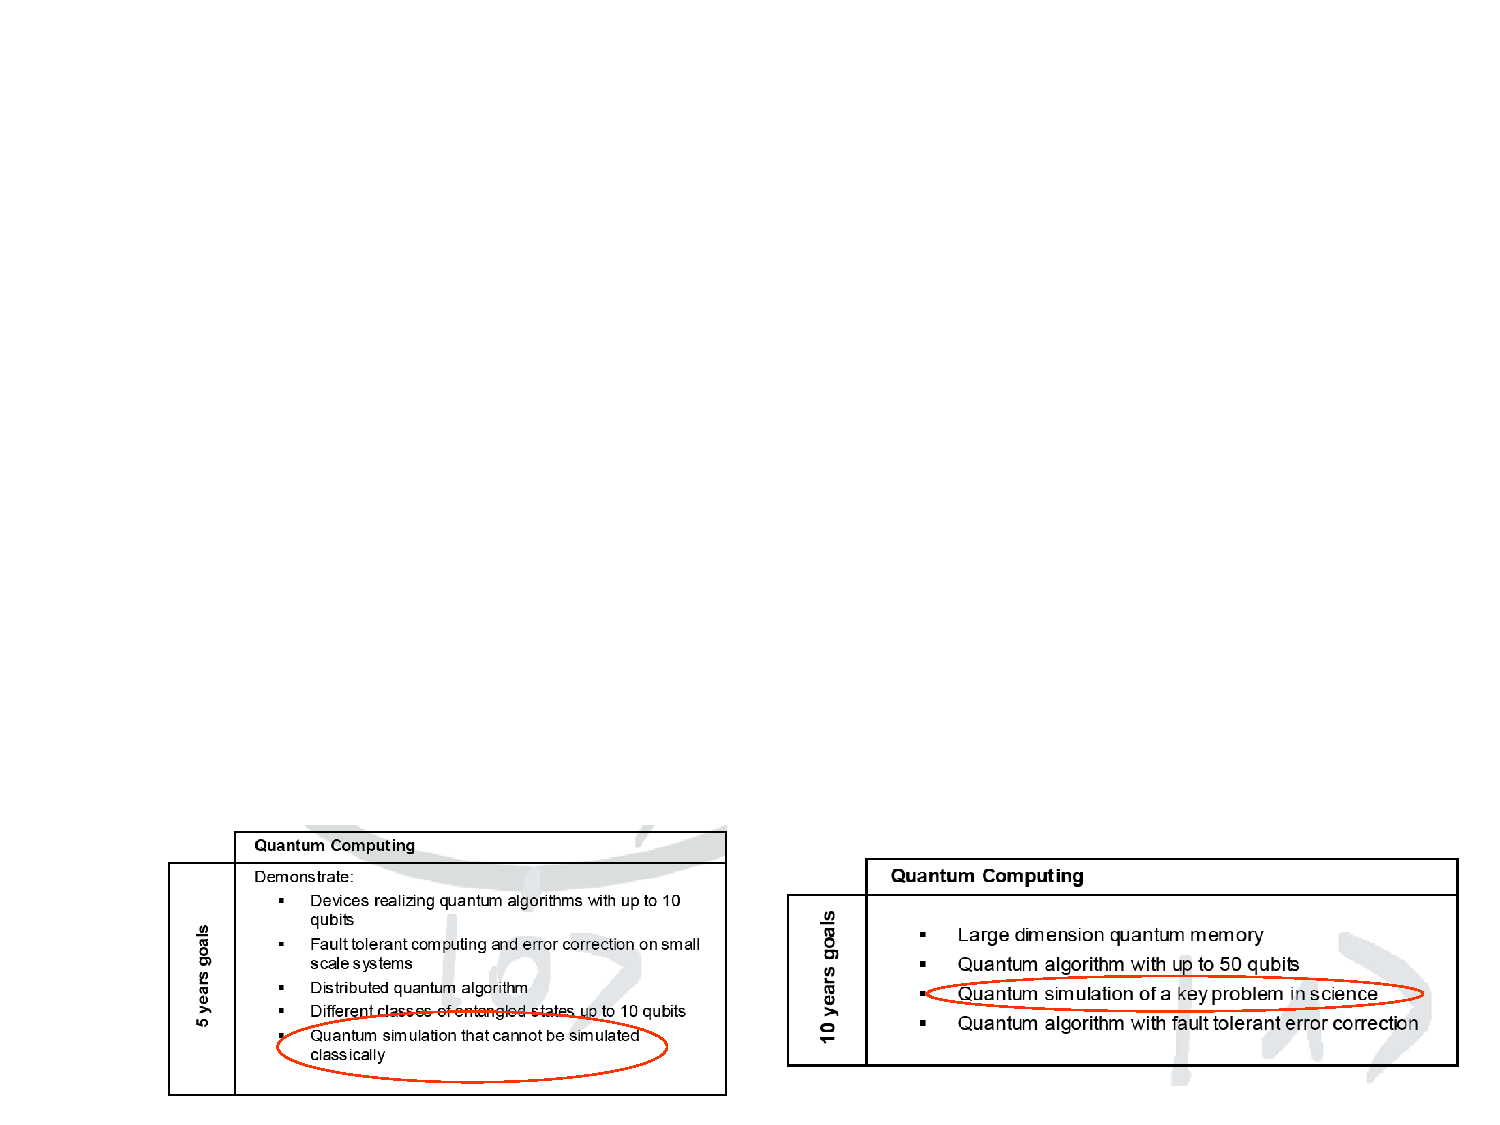
\includegraphics[width= 0.8\columnwidth]{figures/eu.pdf}
              \caption{在2008年欧盟关于量子计算的战略规划中,计划五年之内量子模拟上要找到一个超越经典的例子,而十年内量子模拟要成为科学研究上的一个关键问题。现在距离五年目标它们还剩一年。
              }
              \label{eu}
            \end{center}
        \end{figure}


\subsection{量子模拟的定义}

我们这里给出一个并不十分严格的量子模拟的定义:

   “\emph{量子模拟就是用量子力学的方法来模拟量子系统。}”

也就是说,我们可以通过一个可控的量子系统来模拟其他量子系统\cite{simreview}。假设要模拟的系统的量子态为$\left\vert \phi \right\rangle$,该系统经过幺正演化
\begin{equation}
          U = e^{-iH_{sys}t}
 \end{equation}
从初态$\left\vert \phi(0) \right\rangle$演化到了$\left\vert \phi(t) \right\rangle$。其中,$H_{sys}$是系统的哈密顿量。而量子模拟器中作为一个可控的量子系统,其初态为
$\left\vert \psi(0) \right\rangle$,演化算子为
\begin{equation}
          U' = e^{-iH_{sim}t}.
 \end{equation}
 这里$H_{sim}$是模拟器的哈密顿量,而经过该演化后,模拟器的末态变为$\left\vert \psi(t) \right\rangle$,并且这个态是容易测量的。如果在这两个量子系统间存在一个映射,即$\left\vert \phi(0) \right\rangle$和$\left\vert \psi(0) \right\rangle$,$\left\vert \phi(t) \right\rangle$和$\left\vert \psi(t) \right\rangle$之间存在映射关系,
 那么原量子系统就可以被模拟,其表示可以见图\ref{schematic}。
        \begin{figure}[htbp]
            \begin{center}
              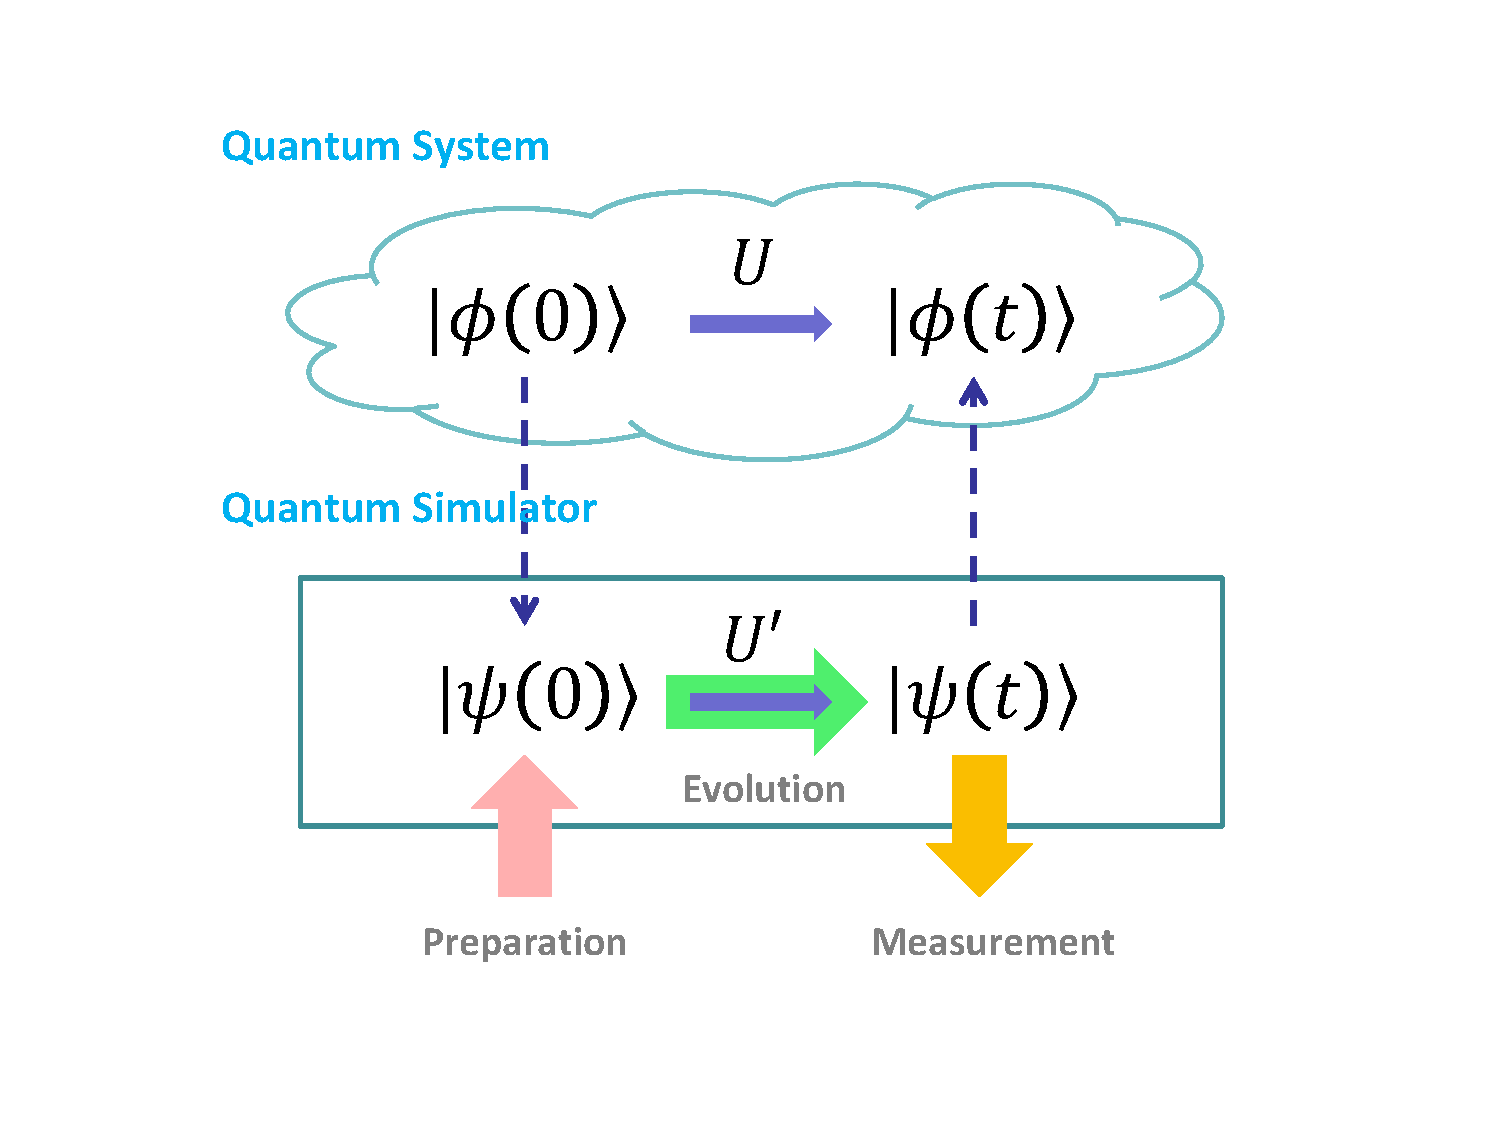
\includegraphics[width= 0.8\columnwidth]{figures/schematic.pdf}
              \caption{量子模拟过程的示意图。量子系统从$\left\vert \phi(0) \right\rangle$经过$U = e^{-iH_{sys}t}$演化到了$\left\vert \phi(t) \right\rangle$,量子模拟器则从$\left\vert \psi(0) \right\rangle$经过$U' = e^{-iH_{sim}t}$演化到$\left\vert \psi(t) \right\rangle$。同时,$\left\vert \phi(0) \right\rangle$和$\left\vert \psi(0) \right\rangle$,$\left\vert \phi(t) \right\rangle$和$\left\vert \psi(t) \right\rangle$之间存在映射关系。虽然量子系统本身不可控制(或者实验上很难控制),但量子模拟器是可以轻易操控的,或者说,初态$\left\vert \psi(0) \right\rangle$容易制备,演化$U'$容易控制,末态$\left\vert \psi(t) \right\rangle$容易测量。有颜色的箭头表示是可控操作。
              }
              \label{schematic}
            \end{center}
        \end{figure}

量子模拟主要分为两类,数字量子模拟(digital quantum simulation, DQS)和类比量子模拟(analog quantum simulation, AQS),这两个概念非常类似于电子学中的数字电路和模拟电路的概念,下面就分别介绍这两种量子模拟形式。

\subsection{数字量子模拟}

为了得到模拟器的末态,我们必须把一个幺正操作作用到初态上,即
\begin{equation}
         \left\vert \psi(t) \right\rangle = U\left\vert \psi(0) \right\rangle  = e^{-iHt}\left\vert \psi(0) \right\rangle.
 \end{equation}
由于$U$可能是多比特的非常复杂的操作,我们一般会用近似把其展开成多个指数项$e^{-iH_lt}$的乘积,其中$H_l$是哈密顿量中的局域相互作用(当然前提是该哈密顿量可以写成
一系列的局域哈密顿量的和的形式)。然后,我们可以利用单比特旋转门和两比特CNOT门把整个$U$展开,就可以得到末态$\left\vert \psi(t) \right\rangle$,从而实现量子模拟任务。这种模拟形式和基于门的量子计算非常类似,也被称作“\textbf{数字量子模拟}”。

理论上,任何的幺正操作总可以用一系列的逻辑门展开,因此原则上来说任何操作都可以被模拟,也就是数字量子模拟是普适的。但实际情况是,并不是所有的幺正操作都可以
有效展开的(仅消耗多项式资源),而且有效拆解逻辑门本身就是一个困难的问题。另外一个问题是,$U$的分解是通过近似方式得到的,所以为了得到高精度的结果,我们必须采用更高阶的近似公式,但
这样做会让逻辑门的个数大量增加。

一般来说,DQS的过程分为以下三步:初态制备,幺正演化及测量读出。下面我们将详细讨论这三个步骤\cite{brown}。

\emph{1. 初态制备}

DQS的第一步就是把量子寄存器从$\left\vert 000\ldots \right\rangle$态上制备到$\left\vert \psi(0) \right\rangle$上。在大多数情况下寻找一个有效的算法是非常困难的,只有一些特定的问题可以做到有效制备初态,比如从一个非对称态出发,可以通过多项式资源
制备到反对称的$n!$个叠加态\cite{ini1};制备$N$个粒子的费米态
\begin{equation}
         \left\vert \psi(0) \right\rangle = \prod_{j=1}^N b_j^{\dagger}\left\vert v \right\rangle,
 \end{equation}
其中$\left\vert v \right\rangle$是真空态,$b_j^{\dagger}$是费米算子\cite{ini2,ini3};有效制备常用的化学波函数\cite{Polynomial_time_algorithm};利用占据$n$个自旋轨道的$m$个电子有效制备分子系统的纯态\cite{ini4}
等等。

        \begin{figure}[htbp]
            \begin{center}
              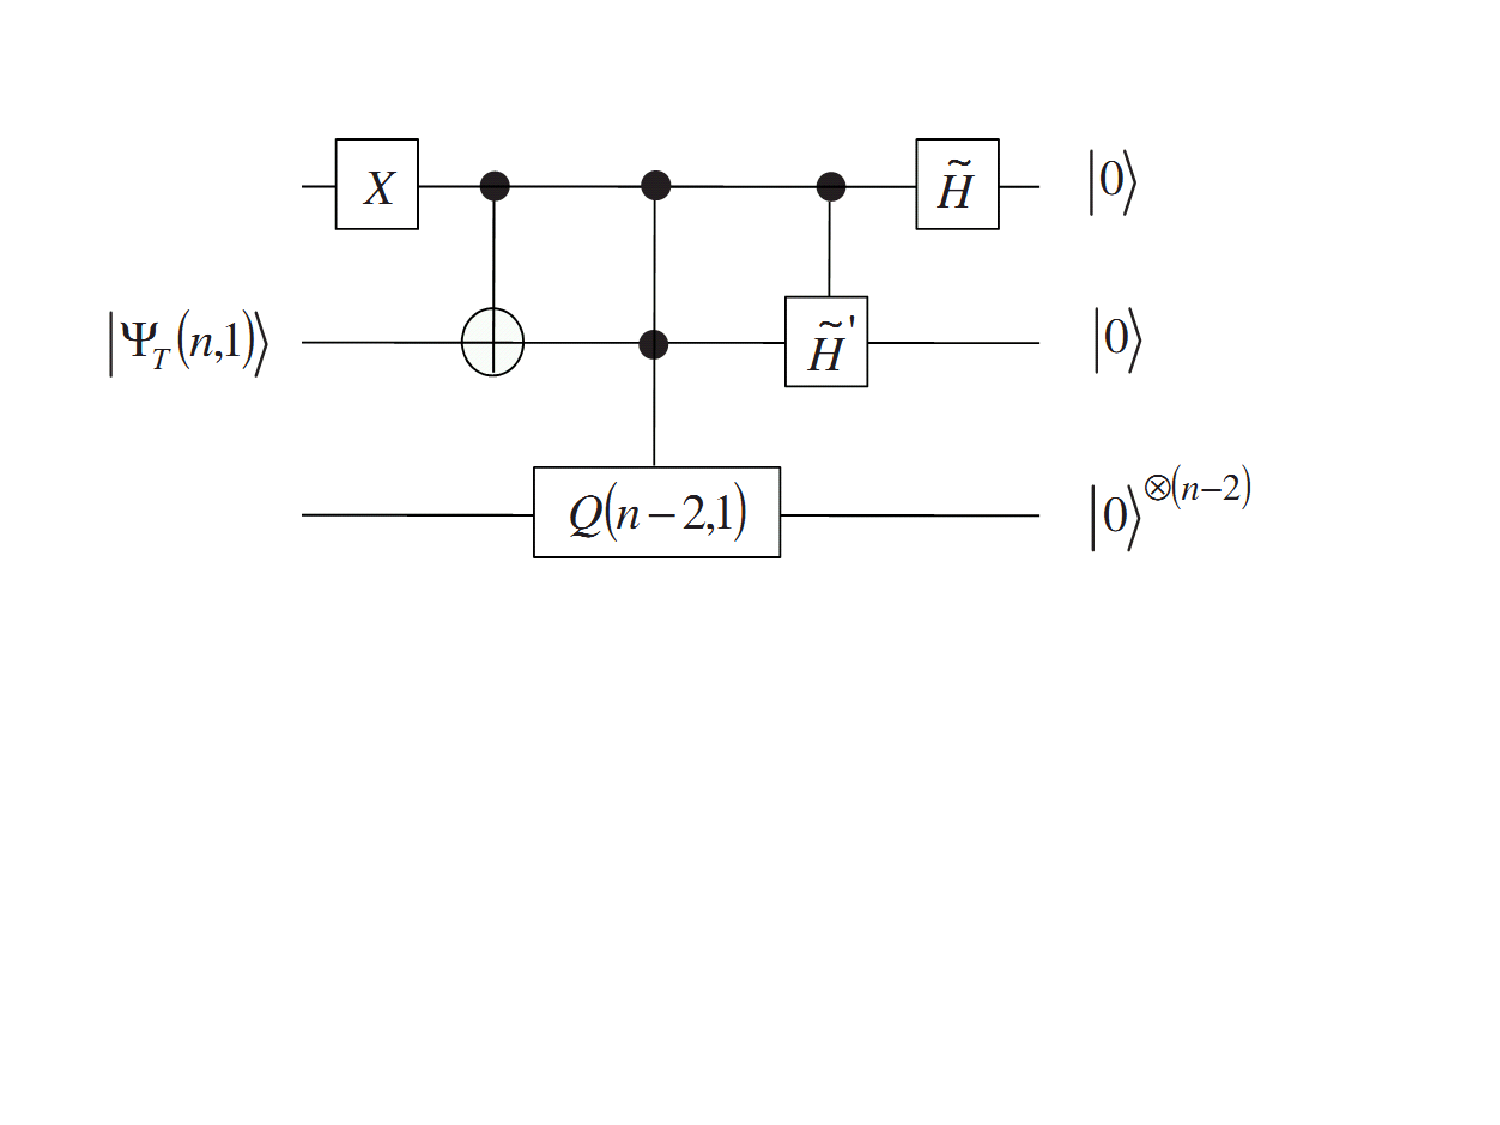
\includegraphics[width= 0.8\columnwidth]{figures/initial.pdf}
              \caption{和一般的初态制备不同,这里的方法是把目标态制备到初态。取自[Phys. Rev. A 79, 042335 (2009)\cite{ini4}
]
              }
              \label{schematic}
            \end{center}
        \end{figure}

\emph{2. 幺正演化}

假设DQS的哈密顿量可以写成一系列局域哈密顿量的和
\begin{equation}
         H = \sum_{l=1}^MH_l,
 \end{equation}
 比如Hubbard和Ising模型的哈密顿量就是这种形式。如果对所有的$l$和$l'$,满足$[H_l, H_{l'}]=0$,那么有
 \begin{equation}
         U = \prod_l e^{-iH_lt}.
 \end{equation}
 否则我们需要用一些近似手段,比如著名的Trotter-Suzuki公式\cite{trotter}
 \begin{equation}\label{trotter}
 U(\delta t)  = \prod\limits_{l=1}^M e^{-iH_l\delta t}+\mathcal {O}(\delta t^2).
\end{equation}
当$\delta t$ 趋近于0时,
 \begin{equation}\label{trotter}
 U(\delta t) \approx  \prod\limits_{l=1}^M e^{-iH_l\delta t}.
\end{equation}
这种方法的缺点是高精度依赖于很小的$\delta t$ ,那么也就会产生大量的逻辑门。目前也有很多文献重新强调Trotter-Suzuki公式的缺点\cite{tro1,tro2}。

\emph{3. 测量读出}

在得到末态$\left\vert \psi(t) \right\rangle = U\left\vert \psi(0) \right\rangle$后,我们必须进行测量来得到需要的信息。一般来说最常用的是量子态重构(tomography)技术,但它并不是可扩展的,所要求的资源也是随着体系的增大
而指数增加的。为了避免这个问题,也有一些方案提出可以利用通过测量特定的物理参数得到想要的信息,比如相关函数或算符谱\cite{ini2},当然这些方法并不是普适的。

比如,为了测量期望值$\langle U^{\dagger}V\rangle$,我们可以通过下图(a)中的线路来实现\cite{mea1}。把一个辅助比特制备到$\left\vert + \right\rangle=(\left\vert 0 \right\rangle+\left\vert 1 \right\rangle)/\sqrt{2}$后,通过网络图演化后我们只需要测量辅助位的期望值$\langle 2\sigma_{+}^a \rangle$就可以得到想要的结果。第二个例子是
描述如何测量一个厄米算符$\hat{Q}$的谱,我们依然可以通过添加辅助位$\left\vert + \right\rangle=(\left\vert 0 \right\rangle+\left\vert 1 \right\rangle)/\sqrt{2}$,并测量辅助位的期望值来实现。

        \begin{figure}[htbp]
            \begin{center}
              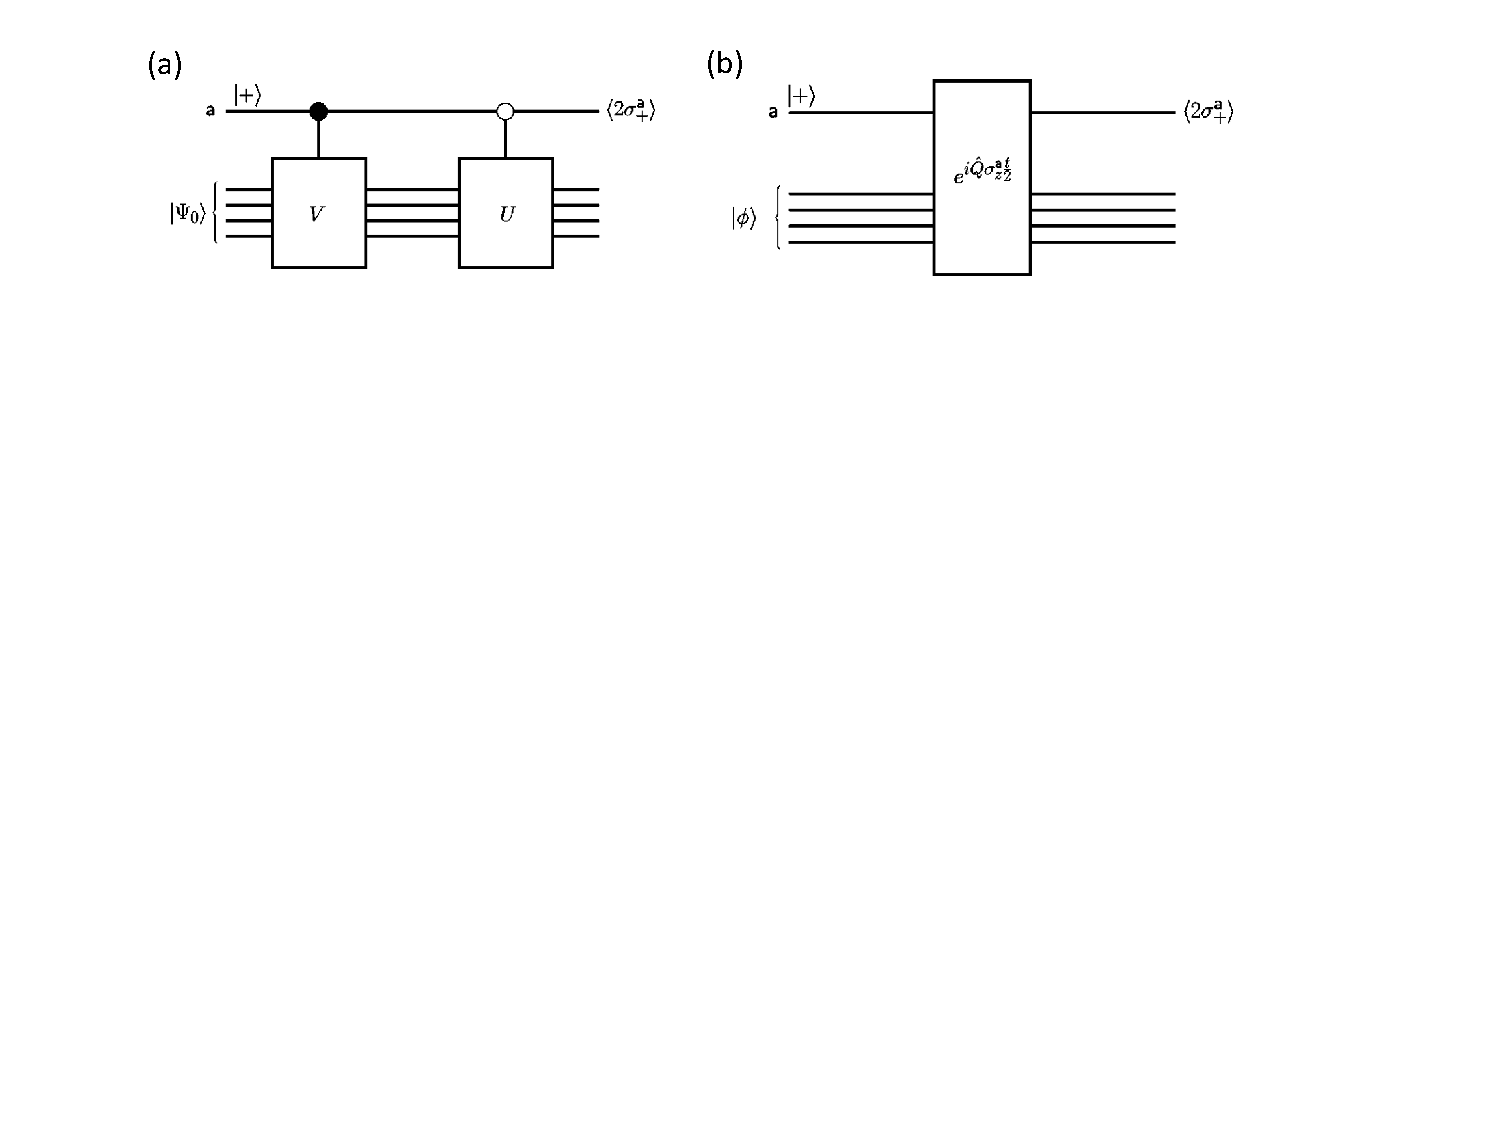
\includegraphics[width= 0.8\columnwidth]{figures/measure.pdf}
              \caption{(a) 测量期望值$\langle U^{\dagger}V\rangle$的线路图。辅助比特制备到$\left\vert + \right\rangle=(\left\vert 0 \right\rangle+\left\vert 1 \right\rangle)/\sqrt{2}$。(b) 测量厄米算符$\hat{Q}$的谱的线路图。取自[Phys. Rev. A 65, 042323 (2002)\cite{mea1}]
              }
              \label{measure}
            \end{center}
        \end{figure}

\subsection{类比量子模拟}

另外一个模拟量子系统的途径就是用类比的方法,也就是“\textbf{类比量子模拟}”。被模拟系统的哈密顿量$H_{sys}$直接映射到模拟器的哈密顿量$H_{sim}$上,也就是
 \begin{equation}\label{trotter}
 H_{sys}\longleftrightarrow H_{sim}.
\end{equation}
一般来说,只有两个量子系统非常相似的时候才能用类比的方法,所以它不是普适的,AQS的模拟精度取决于模拟器重现被模拟系统的演化过程的程度。
尽管不是普适的,AQS吸引人的地方在于它的物理要求较小,并容易在实验上实现。

寻找合适的映射是AQS的核心。一眼看上去,这个过程仿佛要比拆解逻辑门简单许多,但其实两者都很困难。如果模拟器和被模拟系统非常相近,当然AQS的实现会非常直观,遗憾的是
大多数情况并不是这么理想。简单的例子比如描述晶格势场中玻色气体(boson gas)的哈密顿量形式是
 \begin{equation}\label{trotter}
 H_{sim} = -J\sum_{i,j}\hat{a}_i^{\dagger} \hat{a}_j+\sum_i\epsilon_i \hat{n}_i+\frac{1}{2}U\sum_i\hat{n}_i(\hat{n}_i-1),
\end{equation}
其中$\hat{a}_i^{\dagger}$和$\hat{a}_i$对应于第$i$个晶格上的产生和湮灭算符,$\epsilon_i$是第$i$个晶格上由于原子的外部谐振限制产生的能量偏移。$U$是处于单个晶格上
的两个原子间的互斥作用。该哈密顿量模型的形式正好对应于Bose-Hubbard模型
 \begin{equation}\label{trotter}
 H_{BH} = -J\sum_{i,j}(\hat{b}_i^{\dagger} \hat{b}_j+h.c.)-\mu\sum_i \hat{n}_i+\frac{1}{2}U\sum_i\hat{n}_i(\hat{n}_i-1).
\end{equation}
因此这两个系统之间的类比模拟是非常直接的,但是大多数情况下就没这么直观了。

AQS中的初态制备和测量读出至今没有文献进行过详尽讨论。这是因为我们已经假设被模拟体系和模拟器之间已经非常相似,那么初态制备应该是可以有效实现的。同时,
测量模拟器的某些物理参量也可以得到被模拟系统的信息。尽管如此,AQS中的初态制备和测量读出过程依然是以后值得研究的问题。

下图是一个关于DQS和AQS之间的比较:

        \begin{figure}[htbp]
            \begin{center}
              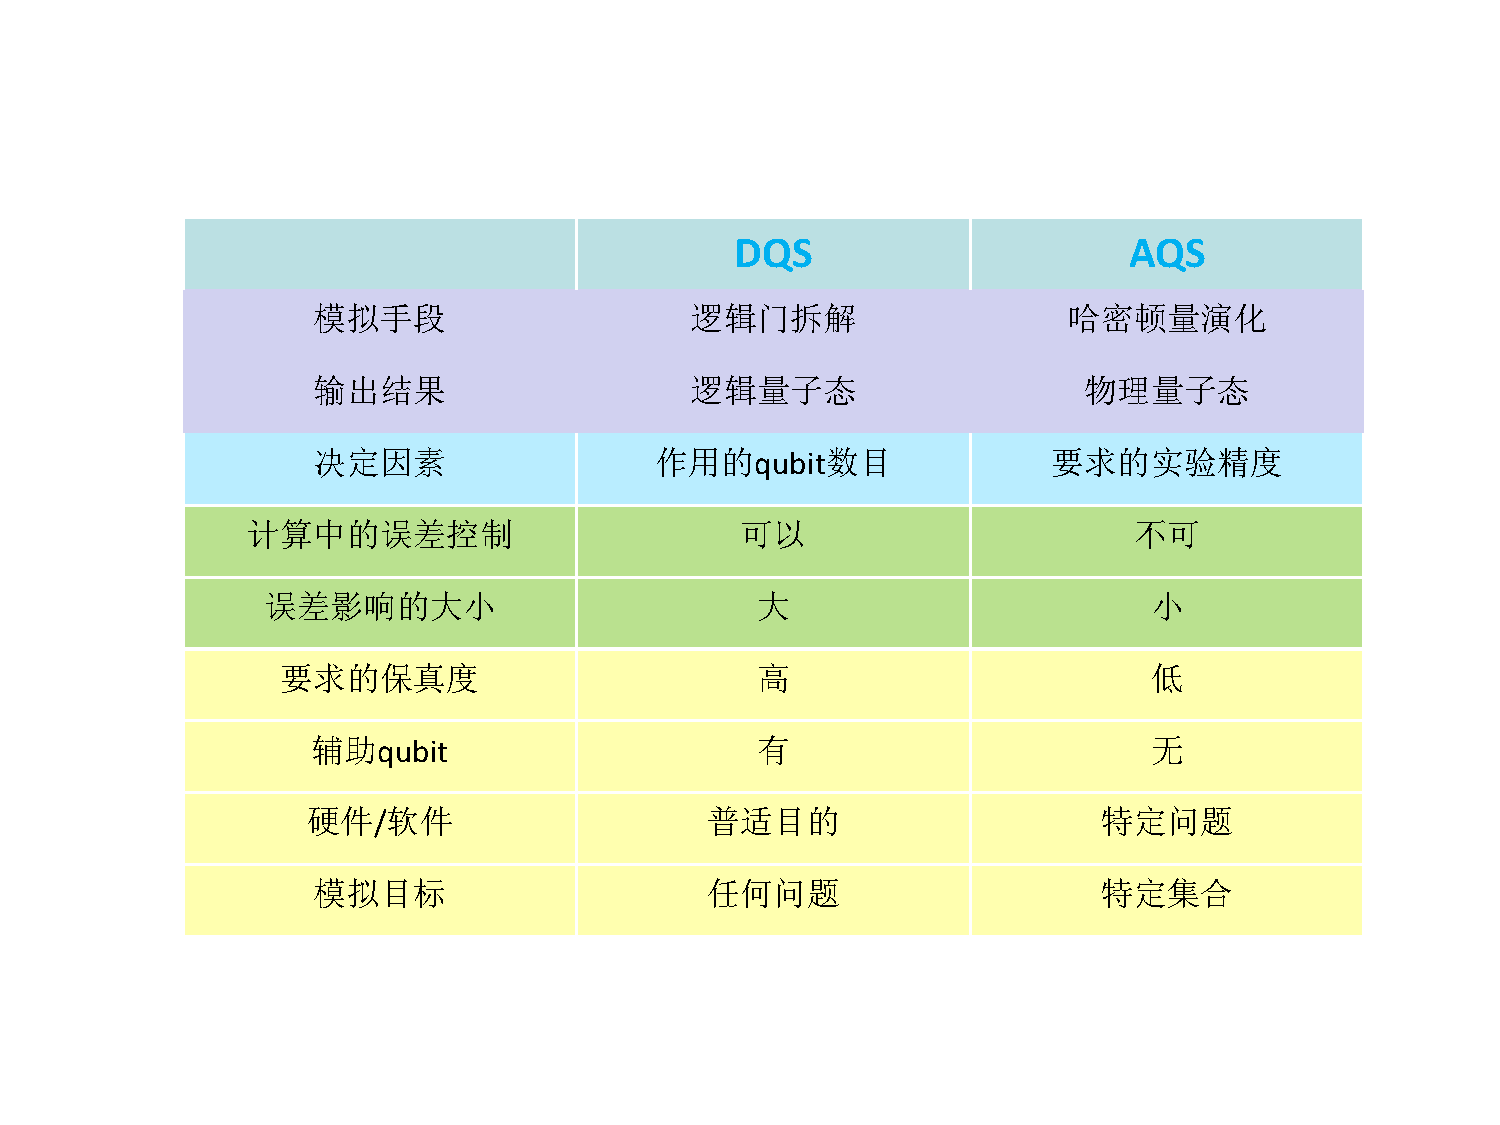
\includegraphics[width= 0.8\columnwidth]{figures/dqsaqs.pdf}
              \caption{DQS和AQS之间的比较。
              }
              \label{dqsaqs}
            \end{center}
        \end{figure}

\subsection{量子模拟的资源要求}

为了实现有效的量子模拟我们到底需要多少个qubit?这个问题的答案依被模拟对象的不同而不同。一般来说AQS对qubit的数目需求较少,当然DQS中也存在一些只用几十个甚至几个qubit
就能解决的问题。例如,在少于十个qubit的情况下,我们可以模拟量子混沌\cite{chaos1,chaos2},化学反应\cite{reaction},Dirac粒子\cite{dirac1,dirac2,dirac},Unruh效应\cite{unruh},任意子\cite{anyons1,anyons2}等等。
而用十几个qubit,我们可以模拟自旋玻璃\cite{glass1,glass2}或者分子能级\cite{Alan_first}。现在认为要超越经典计算的话我们只需要30-100个qubit的量子模拟器\cite{Alan_first}。

一般来说,DQS需要的资源和操控都要高于AQS。而且在DQS中,提高精度的代价是指数增长的逻辑操作\cite{tro1}。不过量子模拟的优势之一就是不需要很高的精度,所以这依然是可以达成的。

我们举一个量子模拟对资源要求的例子:模拟通过双势阱进行相互作用的N个粒子\cite{Polynomial_time_algorithm}。对每个自由度,该模拟都需要$n$个qubit,每个辅助位则需要$m$个qubit,而为了模拟Coulomb势场,又需要4个辅助位。
所以我们一共需要$n(3N-6)+4m$个qubit。Coulomb势场可以用$O(N^2m^2)$步来模拟,因此这个化学反应过程可以用$O(N^2m^2)$模拟,比起经典计算机这已经是指数加速了。
但另一方面来看,为了超越经典计算机我们需要至少100个qubit和200,000个逻辑门!

        \begin{figure}[htbp]
            \begin{center}
              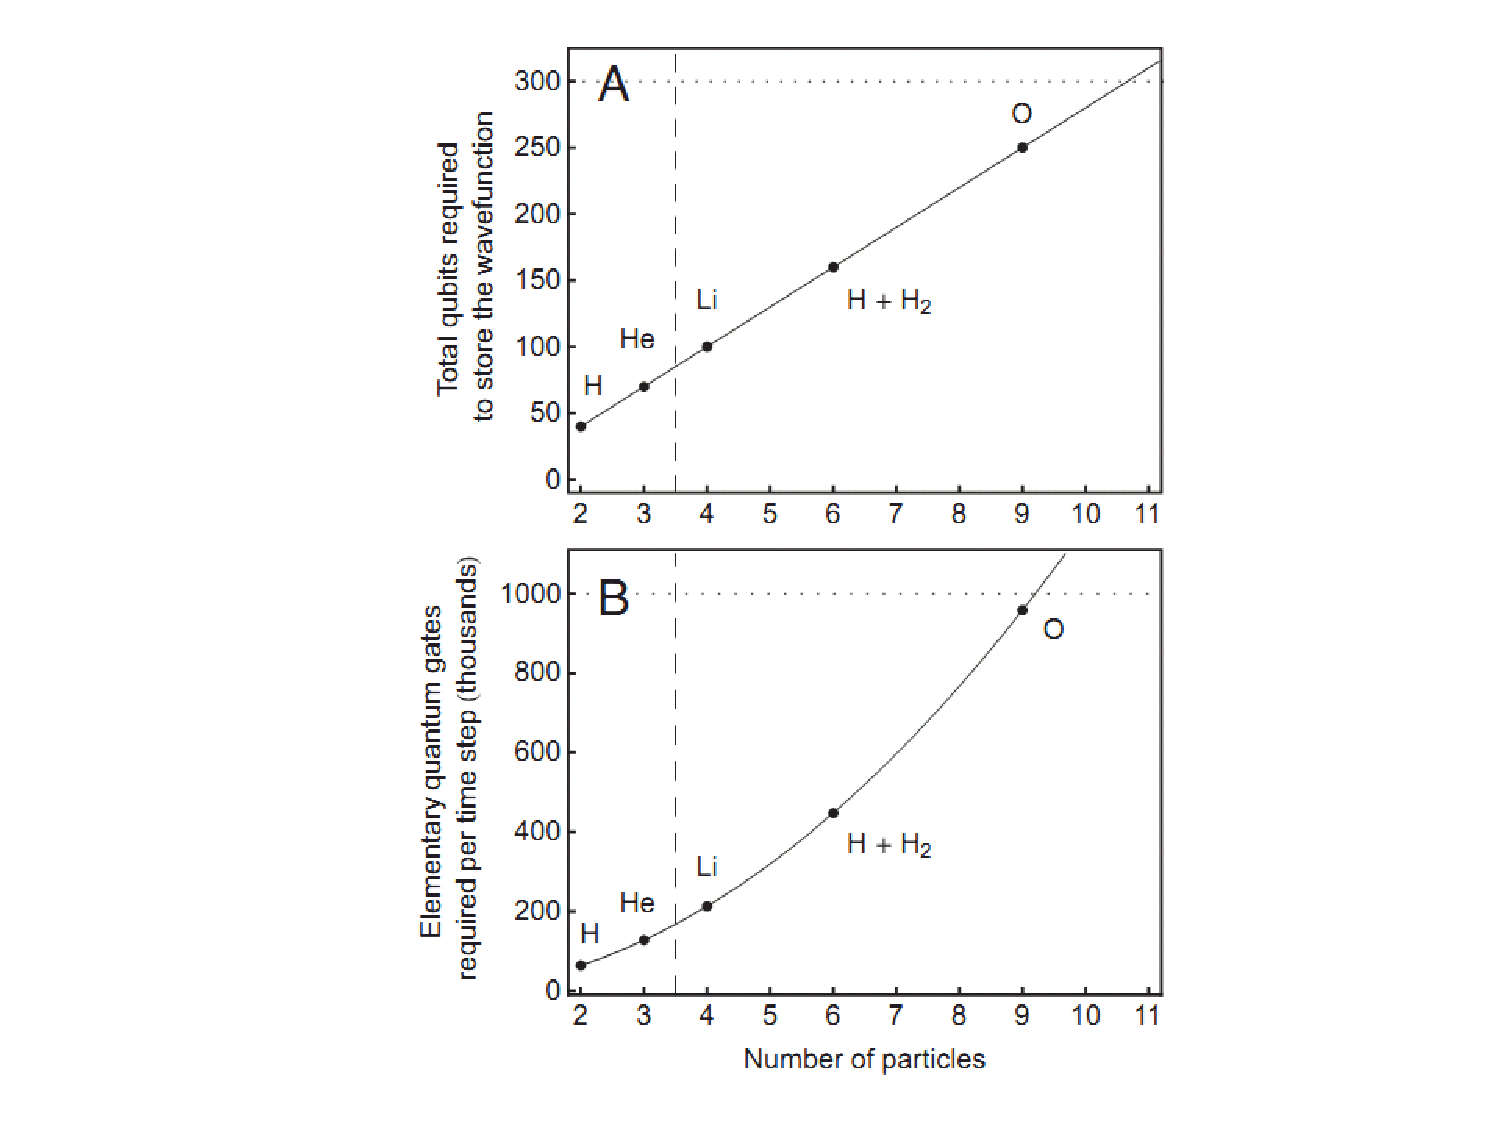
\includegraphics[width= 0.8\columnwidth]{figures/resource.pdf}
              \caption{模拟通过双势阱进行相互作用的N个粒子的资源要求。(a) 需求的比特数:对每个自由度需要$n$个qubit,每个辅助位则需要$m$个qubit,而一共需要4个辅助位,因此总共需要$n(3N-6)+4m$个qubit。水平的虚线代表一个300-qubit的
              量子计算机。(b) 需求的逻辑操作数量。一台300-qubit的量子计算机大概需要十亿个逻辑操作。取自[PNAS 105, 18681  (2008)\cite{Polynomial_time_algorithm}]。
              }
              \label{resource}
            \end{center}
        \end{figure}

\subsection{退相干和纠错}

虽然量子模拟和量子计算和环境的相互作用方式是相似的,但量子模拟中退相干并不是一个非常严重的问题,因为量子模拟需求的精度相对不高。更有趣的是,甚至有
建议模拟器的退相干还可以用来粗略调制被模拟系统的退相干\cite{Lloyd}。Tseng等也通过理论计算和实验证明\cite{deco},在开放系统的量子模拟中可以通过改变被模拟系统和模拟器之间的映射方式来
研究模拟器的退相干机制。原则上,我们可以完全分析退相干是如何影响模拟过程的,然后通过选择合理的映射方式就可以调制模拟器的有效退相干。同时利用子空间的概念
我们也可以减小退相干的影响。而且,理论和实验上也表明退相干可以对临界系统的信息获取有一定的作用\cite{deco1,deco2}。

虽然量子模拟中对精度的要求比量子算法要低,但误差还是要尽量减小的。比如为了模拟薛定谔方程我们要最小化幅度的误差\cite{schro},而对一个局域系统来说其哈密顿量以及所选择qubit的
微小改变都会指数上影响其模拟\cite{mon},而多体相互作用的哈密顿量模型中两体相互作用和局域控制操作的噪声影响也被研究过\cite{dur}。不过总体来说关于这方关于这方面的研究还是偏少。

\section{量子模拟的物理实现}

 “\emph{现代高能物理发展到了量子物理以后,有很多理论根本无法做实验,在家用纸和笔来算已经跟数学家做的差不多了。}”

 \hspace{23em} \emph{--丘成桐}

量子模拟的物理实现要求一个可控的量子系统。对DQS来说,控制的精度要求更高,AQS相对要低一些。理论上,任何可以用作量子计算机的物理系统都可以用来作量子模拟。
反过来,即使不能作为量子计算机的体系也有可能执行AQS,比如BEC中的声波传播子可以用来模拟宇宙膨胀\cite{cosmic}。 当然关于潜在的量子计算方案我们已在第一章讨论过,本节我们将主要关注量子模拟的物理实现。

\subsection{中性原子}

光晶格中的中性原子\cite{atomsim1}非常适合用作模拟凝聚态系统\cite{atomsim2,atomsim3}。自从利用光晶格中的冷原子模拟超流到Mott绝缘体的相变\cite{mott}的第一个实验以来,
中性原子体系模拟凝聚态的工作越来越多。理论和实验的综述性回顾可以分别参见参考文献\cite{atomsim2,atomsim1}。

        \begin{figure}[htbp]
            \begin{center}
              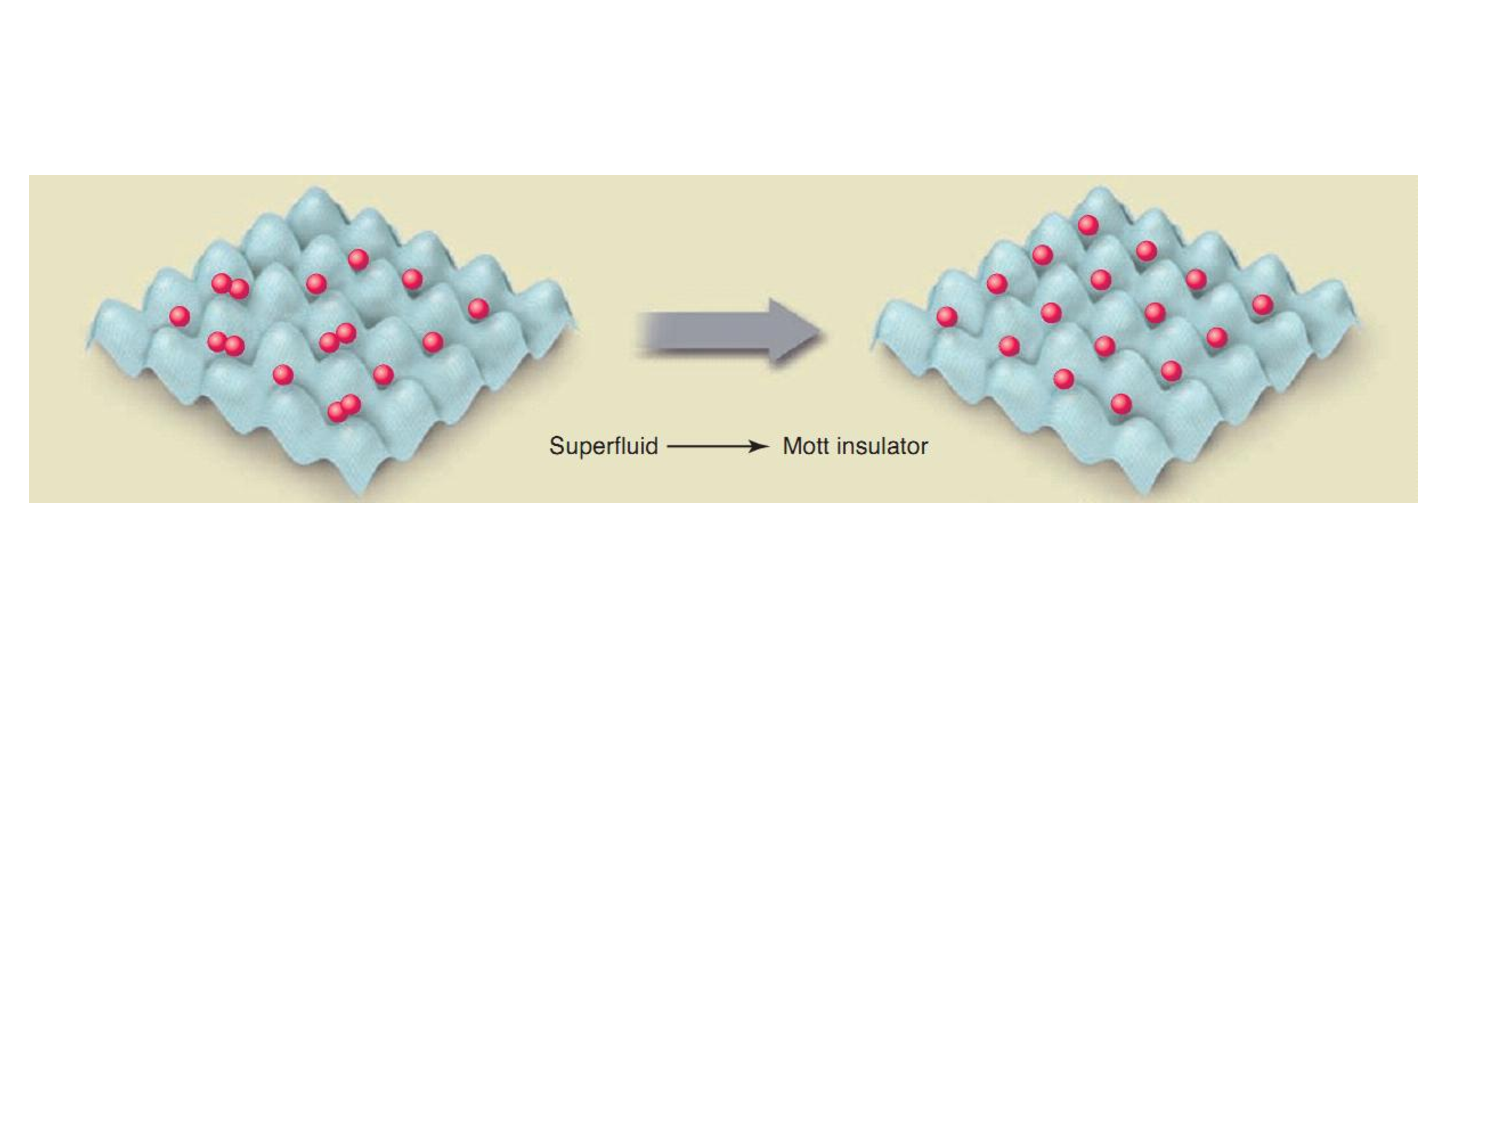
\includegraphics[width= 0.8\columnwidth]{figures/mott.pdf}
              \caption{利用中性原子模拟超流到Mott绝缘体的相变。隧穿能量和本地相互作用能量的比率依靠晶格势场深度来调节,以确保相变发生。取自[Science, 326, 108 (2009)\cite{simreview}]。
              }
              \label{mott}
            \end{center}
        \end{figure}

在中性原子体系中,可调节的参数非常多,所以该系统的使用非常灵活。这些可调节参数包括:隧穿能量,本地相互作用,近邻相互作用,长程相互作用,多粒子相互作用,外部
势场,Rabi振荡等。而光晶格中最常见的哈密顿量形式是Hubbard型\cite{atomsim2}:
 \begin{equation}\label{optical}
 H = H_{hop}+H_{int}+H_{pot}+H_{Rabi},
\end{equation}
其中$H_{hop}$是原子从一个晶格隧穿到另一个晶格的哈密顿量,$H_{int}$是相互作用项,$H_{pot}$是原子感受到的所有势场,$H_{Rabi}$则是原子的内部跃迁哈密顿量。
从这个哈密顿量形式出发很多问题都可以被模拟,包括DQS和AQS。
量子模拟主要通过改变晶格势场的深度或者通过Feshbach共振改变原子-原子间的相互作用来实现,不过光晶格中的单个qubit寻址非常困难,也导致该体系实现一些量子模拟任务时
有些不便。

目前除了模拟超流到Mott绝缘体的相变的实验外,其他的利用中性原子的量子模拟实验包括Tonks-Girardeau Gas的产生\cite{atomsim4}
,BSC-BEC交叉的观测\cite{atomsim5},无序系统的研究\cite{atomsim6,atomsim7}等等。

\subsection{极性分子}

极性分子可以用来模拟拓扑序\cite{polar1,polar2},其优势在于通过控制外加DC和AC的微波场,它的电偶极项可以产生非常强的偶极-偶极相互作用
,非常适合研究强关联系统。利用微波激发,偶极-偶极相互作用,自旋-轨道耦合等,极性分子可以模拟很多自旋模型,包括引申的Hubbard模型\cite{polar3},
量子相变\cite{polar4},或者三角晶格中的超固体(supersolid)相\cite{polar5}等等。关于利用极性分子模拟凝聚态物理的综述性文献可以参见Pupillo等在arXiv上的文章\cite{polar6}。 \begin{figure}[htbp]
            \begin{center}
              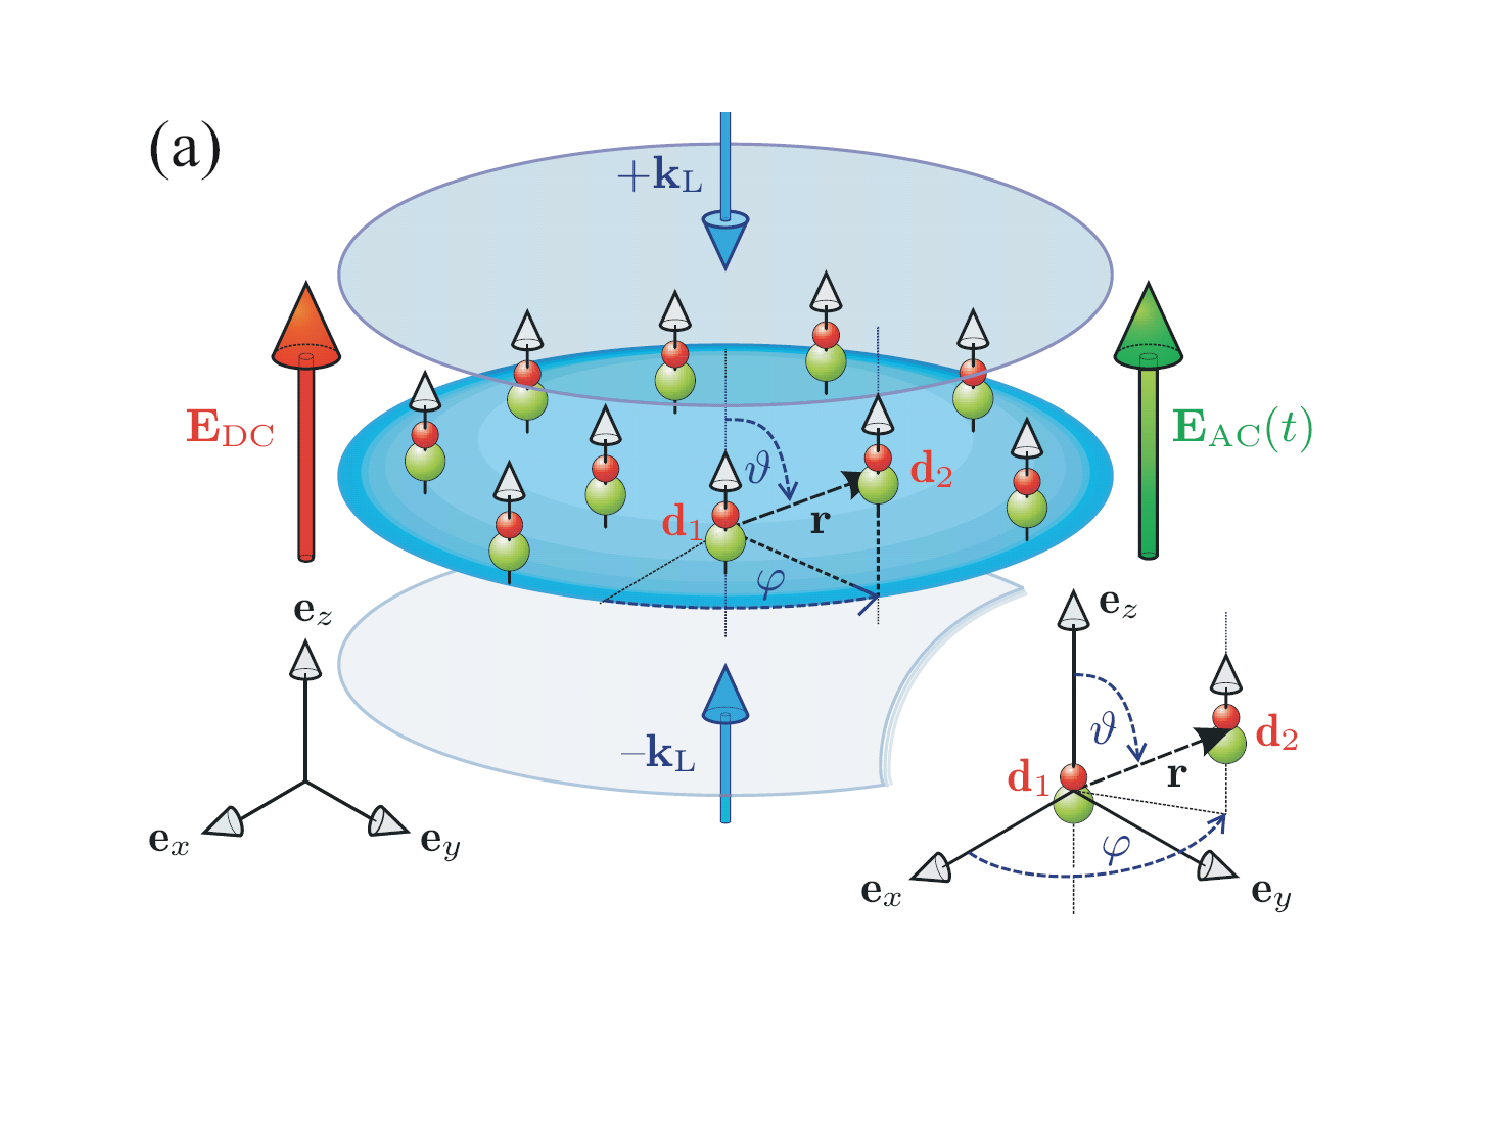
\includegraphics[width= 0.8\columnwidth]{figures/polar.pdf}
              \caption{利用反向传播的激光束可以产生光晶格中的极性分子。蓝色箭头为激光波矢,红色和绿色箭头分别为DC和AC微波场。取自[arXiv:0805.1896 (2008)\cite{polar6}]。
              }
              \label{polar}
            \end{center}
        \end{figure}

\subsection{离子阱}

离子阱体系的哈密顿量形式中可控参数也比较多,因此也可以用作DQS和AQS。利用激光激发将内部能级和振动模式耦合起来的哈密顿量形式为
 \begin{equation}\label{ion}
 H = i\hbar \eta \Omega [e^{i\phi}\sigma_{+}a-e^{-i\phi}\sigma_{-}a^{\dagger}],
\end{equation}
其中$\Omega$是Rabi跃迁频率,$\sigma_{+}$和$\sigma_{-}$是两能级的升降算子,$\eta$是Lamb-Dicke参数,$a^{\dagger}$和$a$是振动模式中
的产生和湮灭算子,$\phi$是激光相位。从这个形式中可以看出单比特门,两比特门甚至三比特门(例如Toffoli)都可以实现。

离子阱中的第一个量子模拟方案可以追溯到1998年\cite{ionsim1},第一个实验则是2002年的非线性干涉仪的模拟\cite{ionsim2}。此外,离子阱还可以用来模拟顺磁性到铁磁
性的相变\cite{ionphase},自旋1/2系统中的对相互作用\cite{ionsim3},相互作用玻色子模型\cite{ionsim4},开放系统\cite{ionsim5},Dirac粒子\cite{dirac},甚至宇宙膨胀中的Unruh效应\cite{unruh}等。

\begin{figure}[htbp]
            \begin{center}
              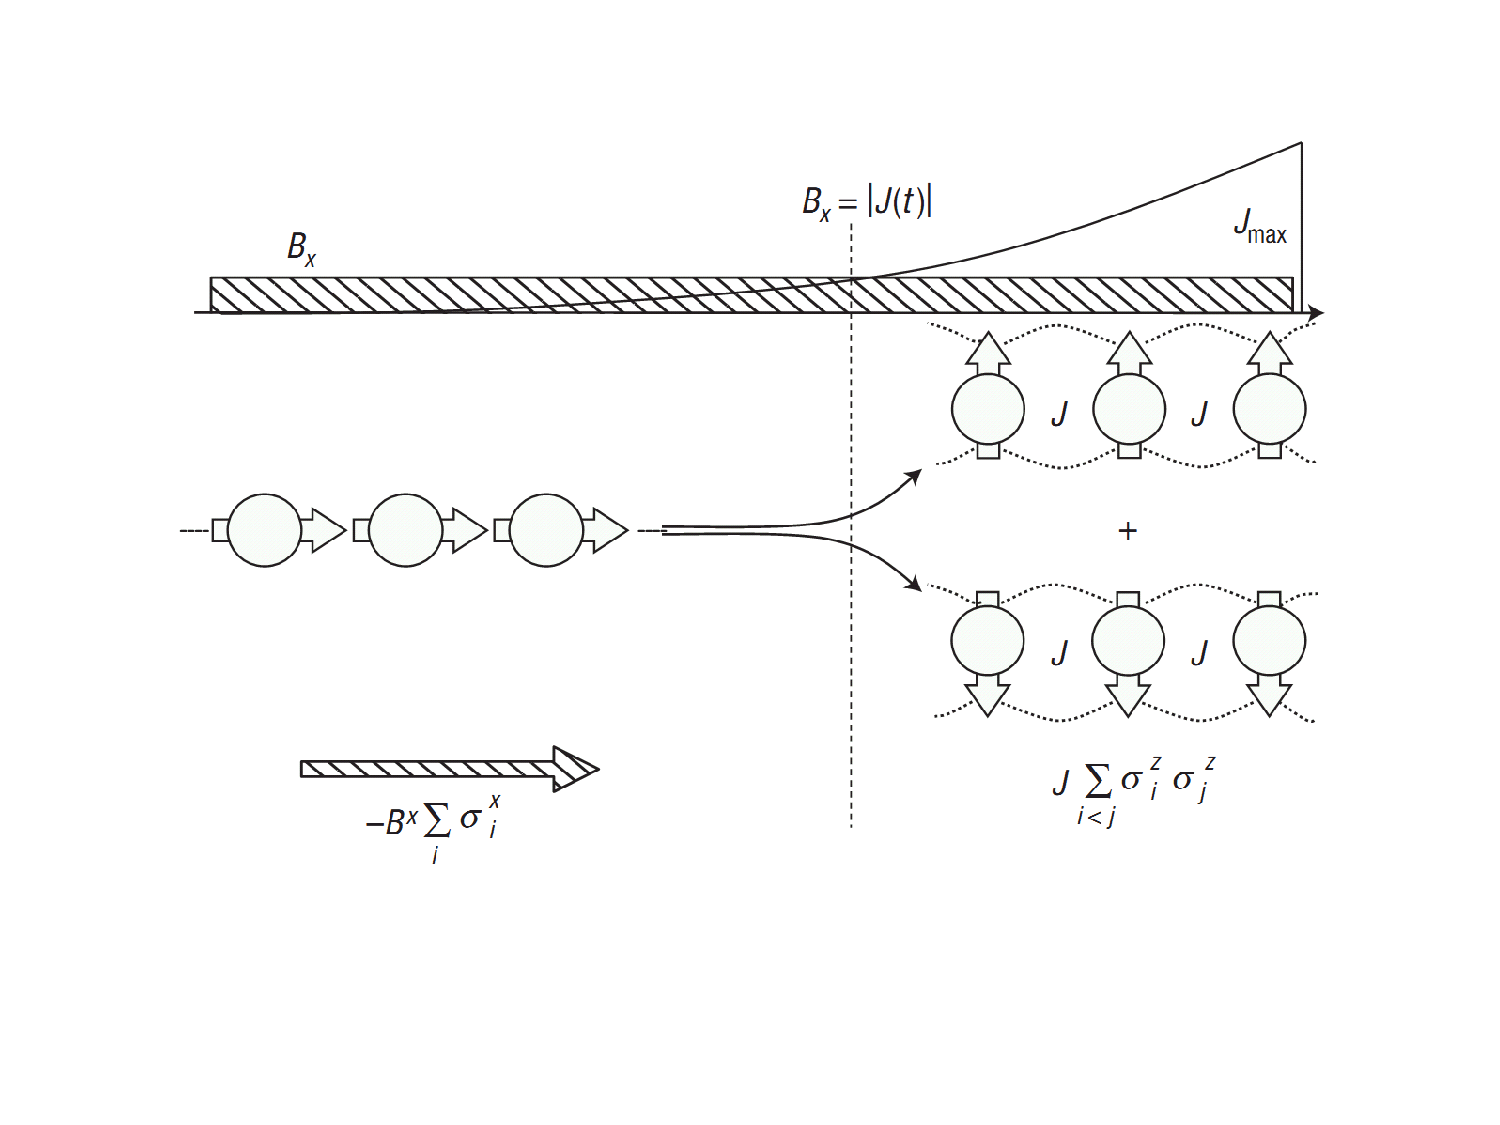
\includegraphics[width= 0.8\columnwidth]{figures/ionsim.pdf}
              \caption{利用离子阱模拟磁性的量子相变。单个自旋依靠射频场把内部能级耦合起来模拟,而自旋-自旋相互作用通过态依赖的光偶极力产生。取自[Nature Phys. 4, 757 (2008)\cite{ionphase}]。
              }
              \label{ionsim}
            \end{center}
        \end{figure}

\subsection{核磁共振}

用核磁共振手段操控的核自旋是最早在实验上执行量子模拟的体系之一。NMR中哈密顿量的形式一般是
 \begin{equation}\label{ion}
 H = -\hbar \gamma I\cdot B+\sum_{i>j}J_{ij} I_i \cdot I_j,
\end{equation}
其中$\gamma$是旋磁比,$I$是角动量算符,$B$是外加磁场,$J_{ij}$是自旋-自旋之间的耦合相互作用。NMR中的技术非常成熟,但它主要的缺点在于可扩展性。
虽然固体NMR在某种意义上可以克服这个问题,但在高维情况下。单比特的寻址以及测量依然非常困难。不过尽管如此,NMR依然非常适合作为小体系量子模拟任务的测试平台,
包括DQS和AQS。

最早的NMR量子模拟实验是利用核自旋模拟谐振子和非谐振子的动力学行为\cite{nmrsim1}。其他的一些实验包括模拟三体相互作用\cite{nmrsim2,app15},开放系统\cite{nmrsim3},量子混沌\cite{chaos2},Fano-Anderson哈密顿量\cite{nmrsim4},
量子相变\cite{nmrsim5,nmrsimphase,app16},哈密顿量对模型\cite{nmrsim6},量子化学等等\cite{static,dynamical,yexiao}。
\begin{figure}[htbp]
            \begin{center}
              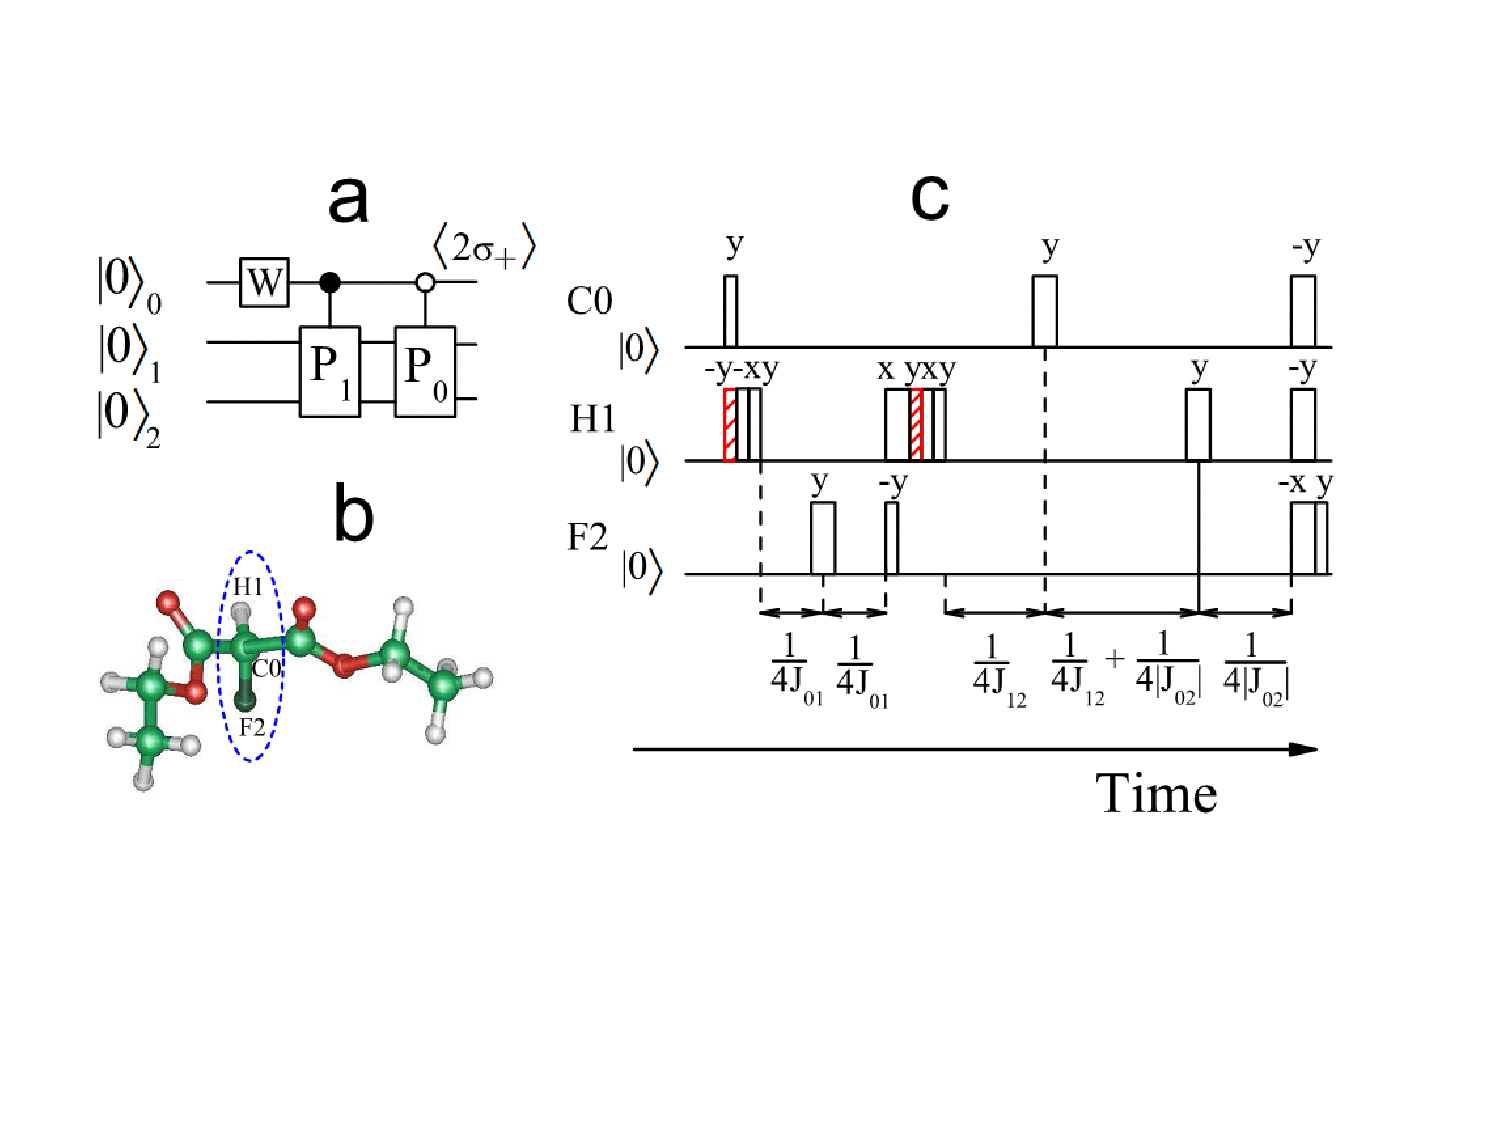
\includegraphics[width= 0.8\columnwidth]{figures/nmrsim.pdf}
              \caption{(a) 利用一个探测qubit测量量子相变的网络图。W是Walsh-Hadamard变换。(b) NMR实验所用的3-qubit样品Diethyl-fluoromalonate。(c) 测量量子态交叠度的脉冲序列图。取自[Phys. Rev. Lett. 100, 100501 (2008)\cite{nmrsimphase}]。
              }
              \label{nmrsim}
            \end{center}
        \end{figure}

\subsection{光子}

由于光子体系的操控灵活性非常低,而且可扩展性也非常有限,所以利用光学体系的量子模拟实验非常少。比较有代表性的工作有
量子混沌\cite{chaos1},任意子的分数统计\cite{anyons1},以及氢分子基态能级模拟的实验\cite{optics_static}。
\begin{figure}[htbp]
            \begin{center}
              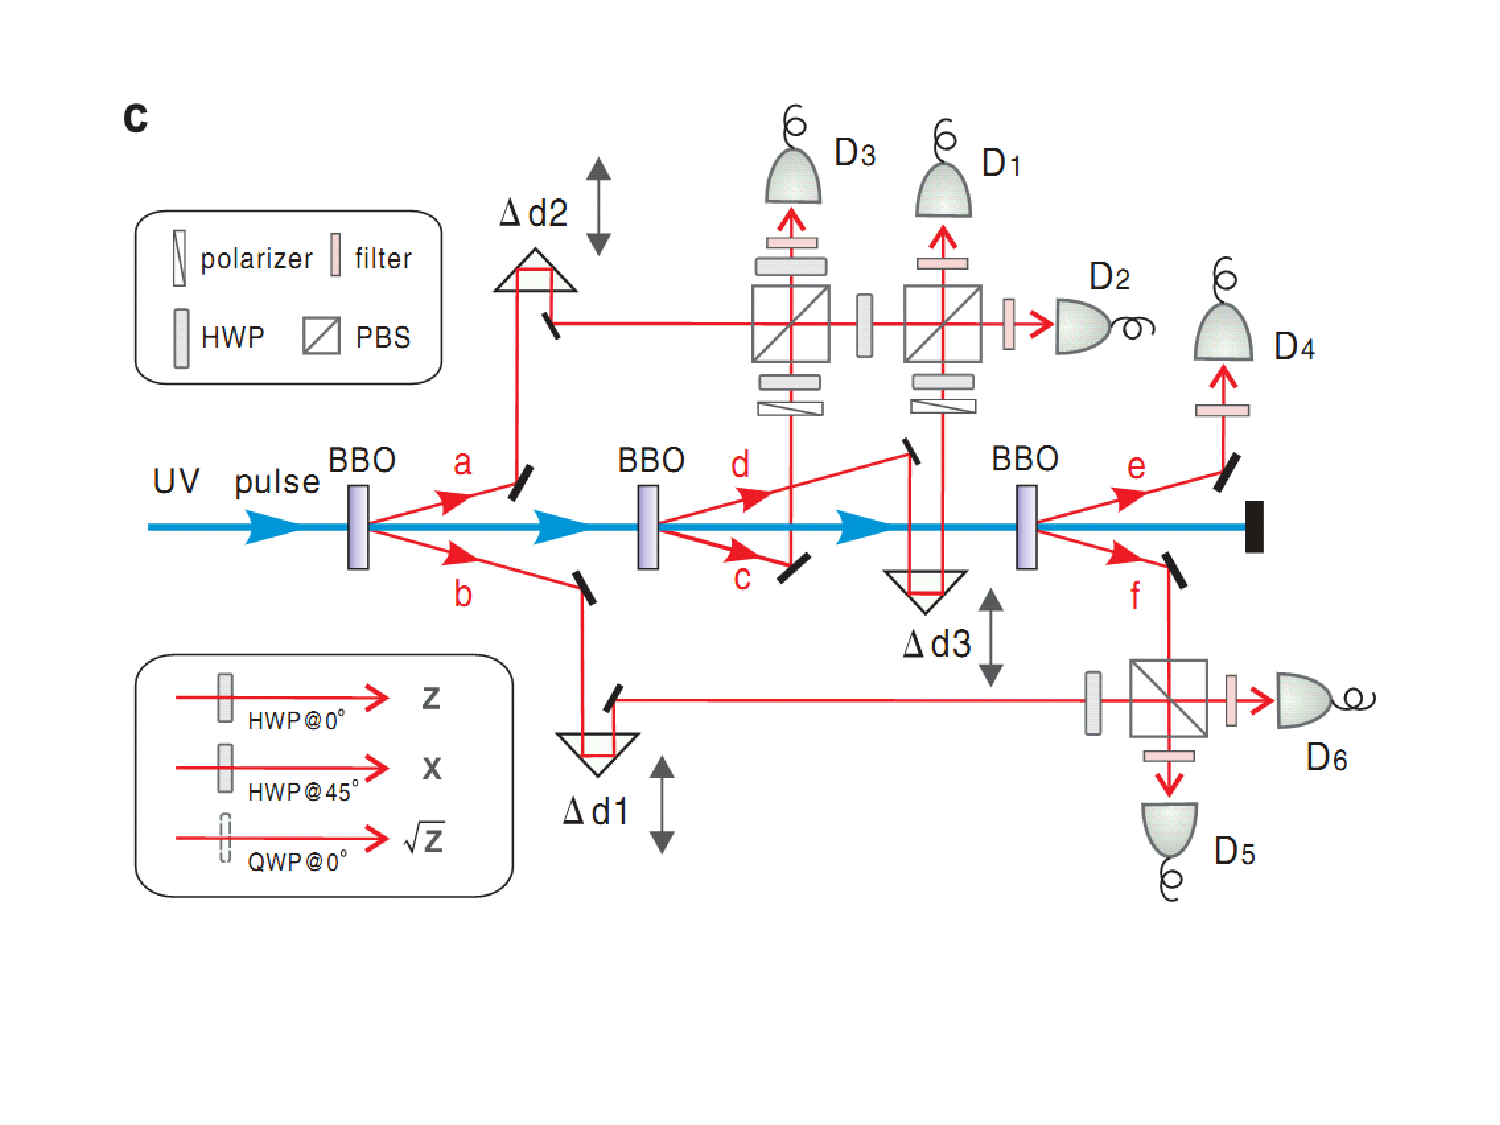
\includegraphics[width= 0.8\columnwidth]{figures/photons.pdf}
              \caption{测量任意子分数统计的实验装置。一束紫外激光通过三个BBO后可以产生三对纠缠的光子。取自[Phys. Rev. Lett. 102, 030502 (2009)\cite{anyons1}]。}
              \label{photons}
            \end{center}
        \end{figure}

\subsection{量子点}

半导体量子点中的电子自旋\cite{dotsim1}也是可以用来作量子模拟的。由于量子点是半导体器件,其激发被限制在一维或二维的很小的区域上。一旦该区域的大小和电荷载体的波长大致
相等,就有了分离的能级结构,此时量子点的行为就非常类似于一个真正的原子。同时,量子点的操控也比较灵活,而且技术上用光激发也比较容易,因此是非常合适的
实验量子模拟体系。量子点的哈密顿量一般形式为
 \begin{equation}\label{dotsim}
 H = \sum_{j=1}^n\mu_B g_j(t) B_j(t)\cdot S_j +\sum_{1\leq j<k\leq n} J_{jk}(t)S_j\cdot S_k,
\end{equation}
其中第一个求和项是外加磁场引起的能量,第二个求和项是加在量子点之间的栅电压产生的隧穿效应引起的相互作用哈密顿量。相对于囚禁在光晶格中的原子,
量子点的接近Fermi温度的极低温要求可以实现自然的长程Coulomb相互作用\cite{dotsim2}。

量子点中可以执行的量子模拟任务有Fermi-Hubbard模型\cite{dotsim2},高温超导体中的CuO平面\cite{dotsim3},甚至化学反应\cite{reaction}等等。 \begin{figure}[htbp]
            \begin{center}
              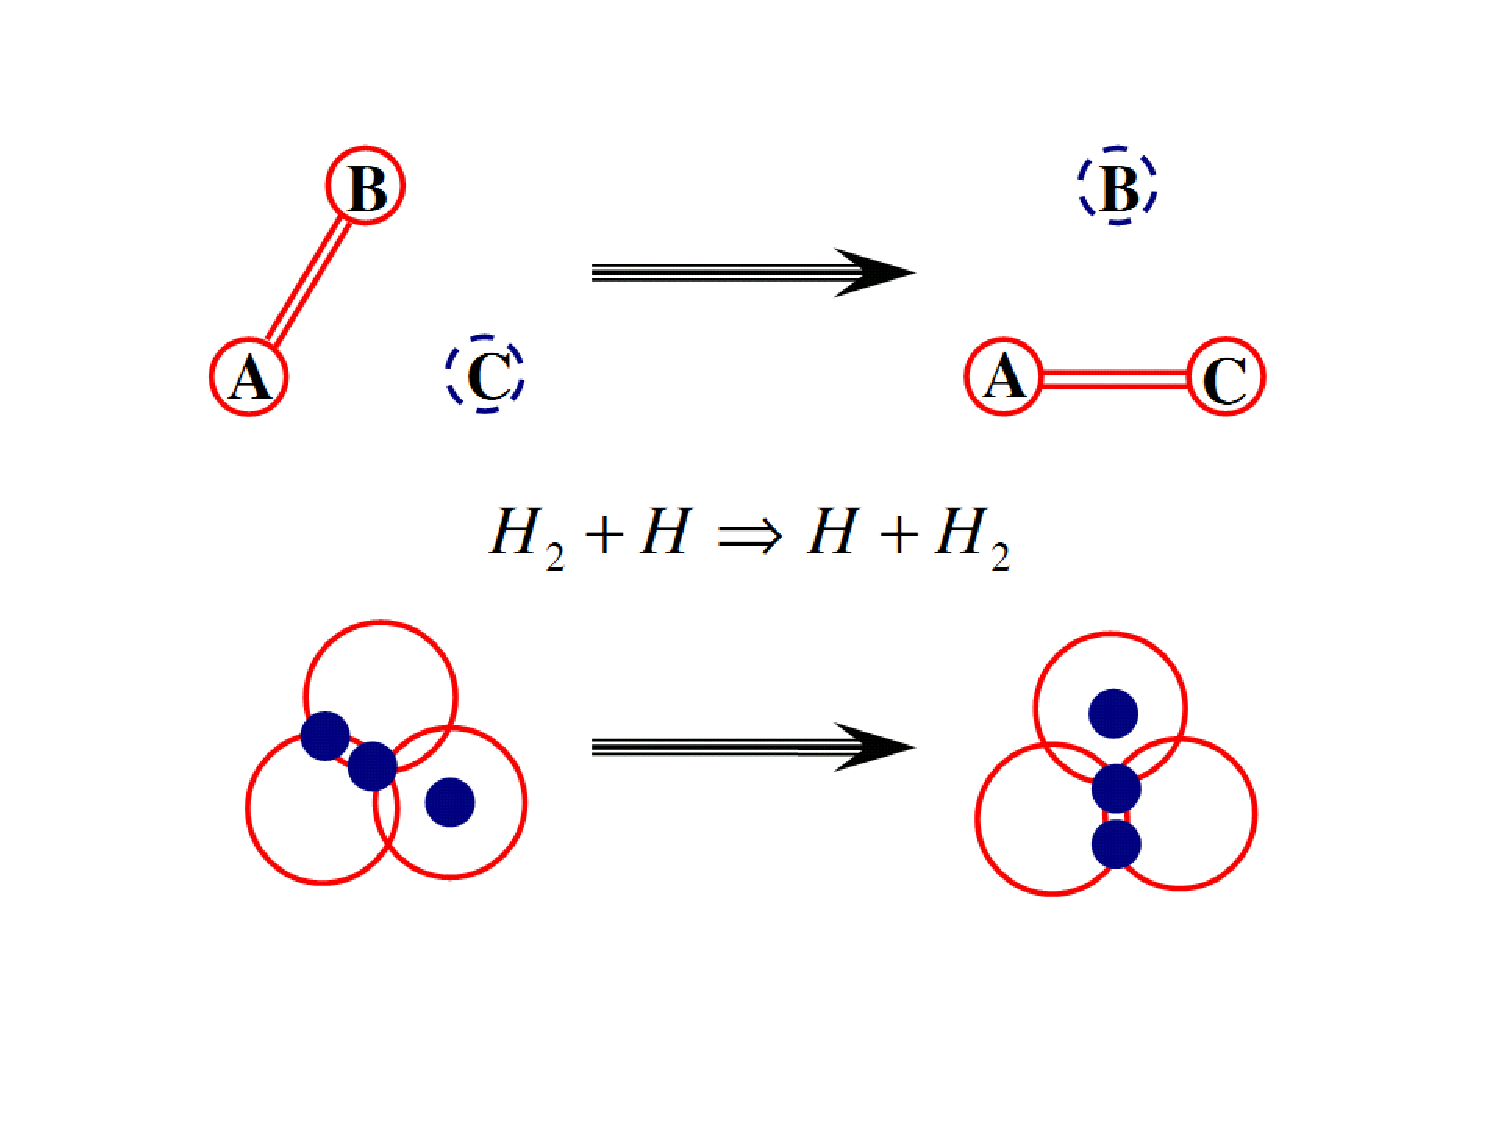
\includegraphics[width= 0.8\columnwidth]{figures/dotsim.pdf}
              \caption{H$_2$+H$\longrightarrow$H+H$_2$化学反应的示意图(上半部分)以及耦合量子点系统中
              电子的重新分配(下半部分)。取自[Euro. Phys. Lett. 80, 67008 (2007)\cite{reaction}]。
              }
              \label{dotsim}
            \end{center}
        \end{figure}

\subsection{超导线路}

虽然超导线路是肉眼可见的,但它表现出了很强的量子行为,因此可以被理解为“模拟原子”。和真正的原子比起来,超导线路中的特征频率和一些其他参数都可以被
精心设计和构造,比如共振频率可以通过外加参数调制,耦合强度则可以依据实验要求随时开关。通过电容(电感)耦合起来的电荷(磁通)qubit的哈密顿量可以写成
 \begin{equation}\label{supersim}
 H = -\sum_{i=1}^N \frac{\Delta_i}{2} \sigma_i^z-\sum_{i,j}J_{ij} \sigma_i^x\sigma_j^x,
\end{equation}
其中$\Delta_i>0$是能级劈裂,$J_{ij}$是耦合强度。超导线路中的单个比特控制和测量都已经解决的很好,但可扩展性问题依然有待解决。

除了最早的观测通过量子涡流形成的一维Mott绝缘体\cite{supersim1}的工作外,超导线路还可以用来模拟原子物理和量子光学中\cite{supersim5}的许多现象,蜂巢状晶格上的Kitaev模型\cite{supersim2},Anderson和Kondo模型\cite{supersim3},
可调材料\cite{supersim4}等等。

\begin{figure}[htbp]
            \begin{center}
              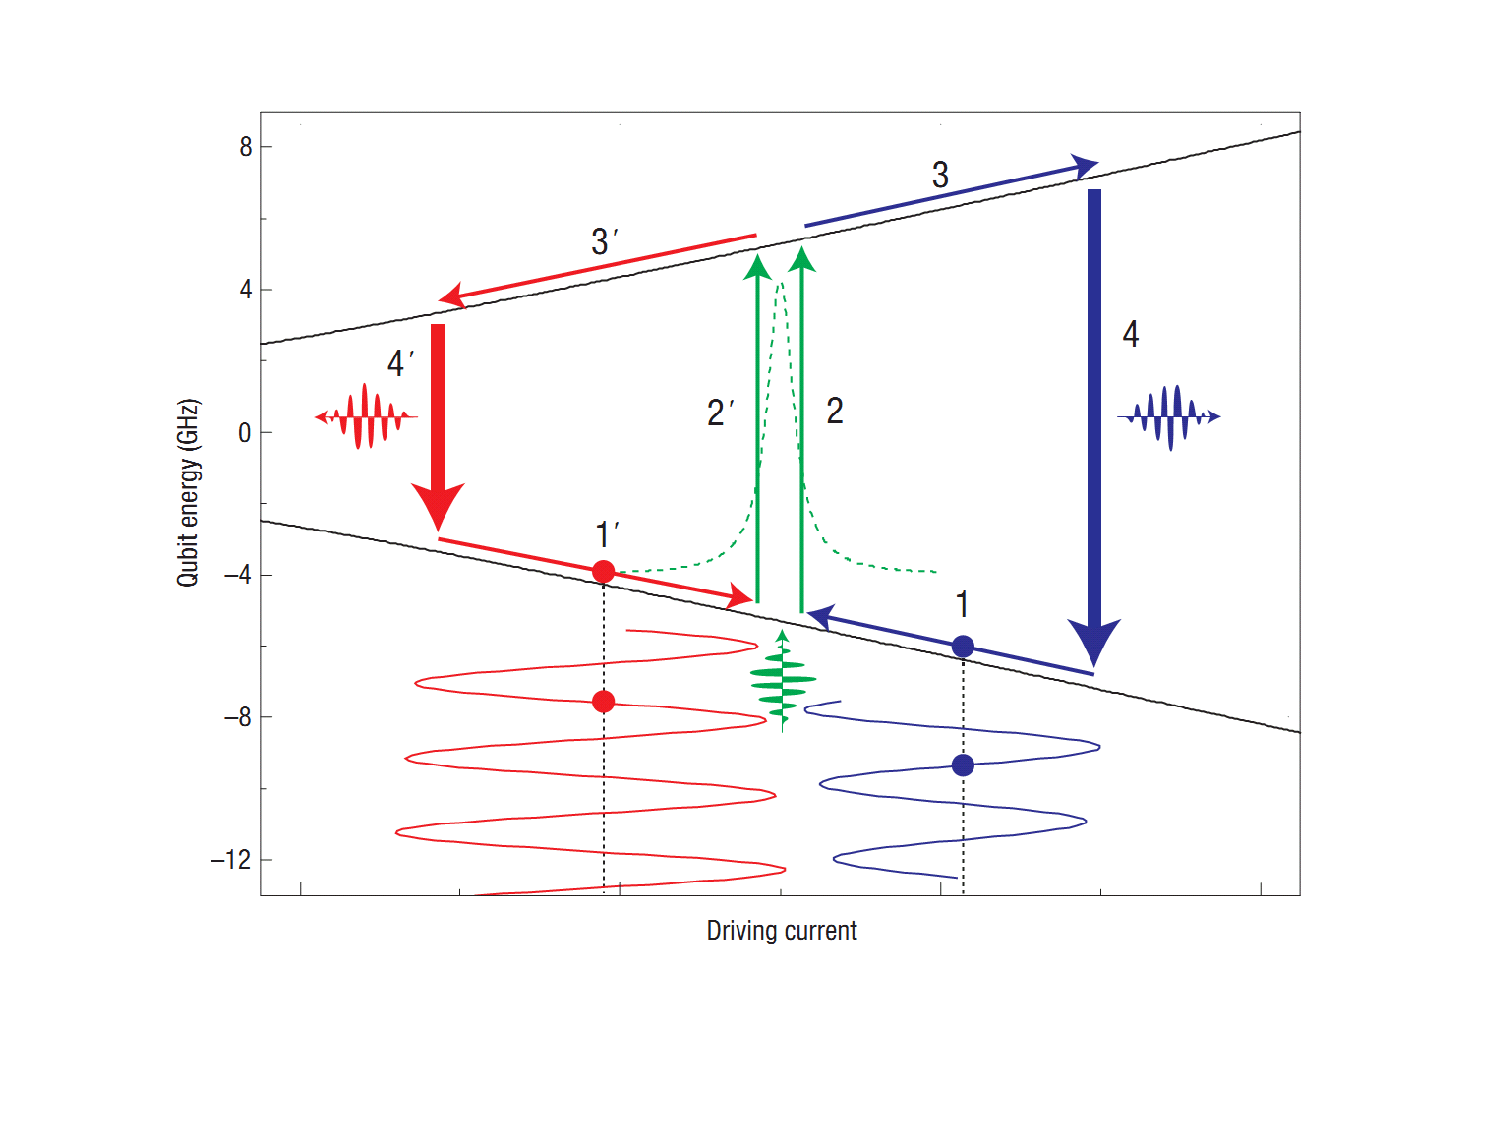
\includegraphics[width= 0.8\columnwidth]{figures/supersim.pdf}
              \caption{利用介观线路模拟Sisyphus(希腊神话中的科林斯王)冷却。$1\longrightarrow2\longrightarrow3\longrightarrow4$的循环
              模拟了原子物理中的Sisyphus冷却,以及希腊神话中科林斯王的命运。取自[Nature Phys. 4, 589 (2008)\cite{supersim5}]。
              }
              \label{supersim}
            \end{center}
\end{figure}

 \section{量子模拟的应用}

  “\emph{每引入一个方程式,就会使读者减少一倍。}”

 \hspace{23em} \emph{--史蒂芬·霍金}

从前面对量子模拟领域的介绍来看,量子模拟至少在物理和化学上肯定有很广泛的应用。不仅如此,它在生物和材料学,甚至宇宙学上也能解决一些经典计算上难以
处理的问题。特别的,如果是模拟量子系统,量子模拟器更是可以预言一些新结论,测试一些新模型,而这些都是经典模拟方法做不到的。本节我们就将介绍
到底有哪些困难的问题可以用量子模拟解决。

 \subsection{凝聚态物理}

 凝聚态物理中存在非常多种经典上难以处理的多体问题,下面我们将具体讨论这些问题。

 \emph{1. Hubbard模型}

 对于存在于一个晶格上的相互作用的粒子来说,Hubbard模型是最简单的模型。但是,在大量粒子及高维的情况时,这个问题就很难在经典上处理了。
 通过DQS我们可以有效模拟Hubbard模型。针对如何获得费米Hubbard哈密顿量的能级谱
 \begin{eqnarray}\label{supersim}
 H_H &=& -\sum_{(i,j);\sigma}[t_x(a^{\dagger}_{(i,j);\sigma}a_{(i+1,j);\sigma}+a^{\dagger}_{(i+1,j);\sigma}a_{(i,j);\sigma})+t_y(a^{\dagger}_{(i,j);\sigma}a_{(i,j+1);\sigma}+a^{\dagger}_{(i,j+1);\sigma}a_{(i,j);\sigma})]\nonumber \\
 &&+U\sum_{(i,j)}n_{(i,j);\uparrow} n_{(i,j);\downarrow},
\end{eqnarray}
Somma等详细讨论了该模型与DQS之间的映射,以及初态制备,演化,测量等所有步骤\cite{mea1}。同时,该模型在Ho等人的工作中也有讨论\cite{hubbard1}。

当然,该模型也可以用AQS的思想来研究,比如在量子点中\cite{dotsim2},极性分子中\cite{polar3}以及离子阱\cite{ionsim4}中都有涉及Hubbard模型。

 \emph{2. 量子相变}

 当一个物理参量在绝对零度下发生改变时,量子相变就可能发生,它描述的是一个多体系统中因为量子涨落导致的基态能级突变。量子相变是非常基础但非常重要的领域之一,
 可惜在经典上模拟或者实验都非常困难,而对量子相变的深入研究会提高我们对纯净量子现象的认识。量子模拟实验第一个观测到的相变是利用光晶格中的中性原子模拟从超流到Mott绝缘体的相变\cite{mott},
 前面已经有了详细介绍,这里不再赘述。

 另外一种相变的粒子是量子磁性的相变,比如离子阱中利用绝热手段模拟的量子顺磁性到反铁磁性的相变\cite{ionphase},该工作利用离子阱平台重复了我们在NMR系统中的量子相变模拟工作\cite{nmrsim5}。该系统可以用简单的Ising模型描述
 \begin{equation}\label{supersim}
 H_I = -B_x\sum_i \sigma_i^x+\sum_{i<j}J_{ij}\sigma_i^z\sigma_j^z,
\end{equation}
其中$B_x$是磁场强度,$J_{ij}$是自旋-自旋相互作用。通过绝热改变相互作用强度,同时保持外磁场$B_x$为常数,我们可以观测到系统从一个顺磁性状态
$\left\vert \rightarrow \right\rangle \left\vert \rightarrow \right\rangle$变到一个反铁磁性状态$\left\vert \uparrow \right\rangle \left\vert\uparrow \right\rangle+\left\vert \downarrow \right\rangle \left\vert\downarrow \right\rangle$。

  \emph{3. 自旋模型}

 考虑最简单的Heisenberg自旋哈密顿量模型
  \begin{equation}\label{supersim}
 H_{XYZ} = \sum_{i=1}^N[J_x\sigma_i^x\sigma_{i+1}^x+J_y\sigma_i^y\sigma_{i+1}^y+J_z\sigma_i^z\sigma_{i+1}^z].
\end{equation}
在离子阱中,XY以及XYZ模型相互作用都已通过利用集体振动模式实现\cite{model1},自旋链和自旋梯的模型也已在光晶格中被讨论\cite{model2};高维或者不规则维度
的自旋模型则被认为可以在超导线路中模拟\cite{model3};反铁磁的Heisenberg模型则可以通过固态NMR实现\cite{model4}。

\begin{figure}[htbp]
            \begin{center}
              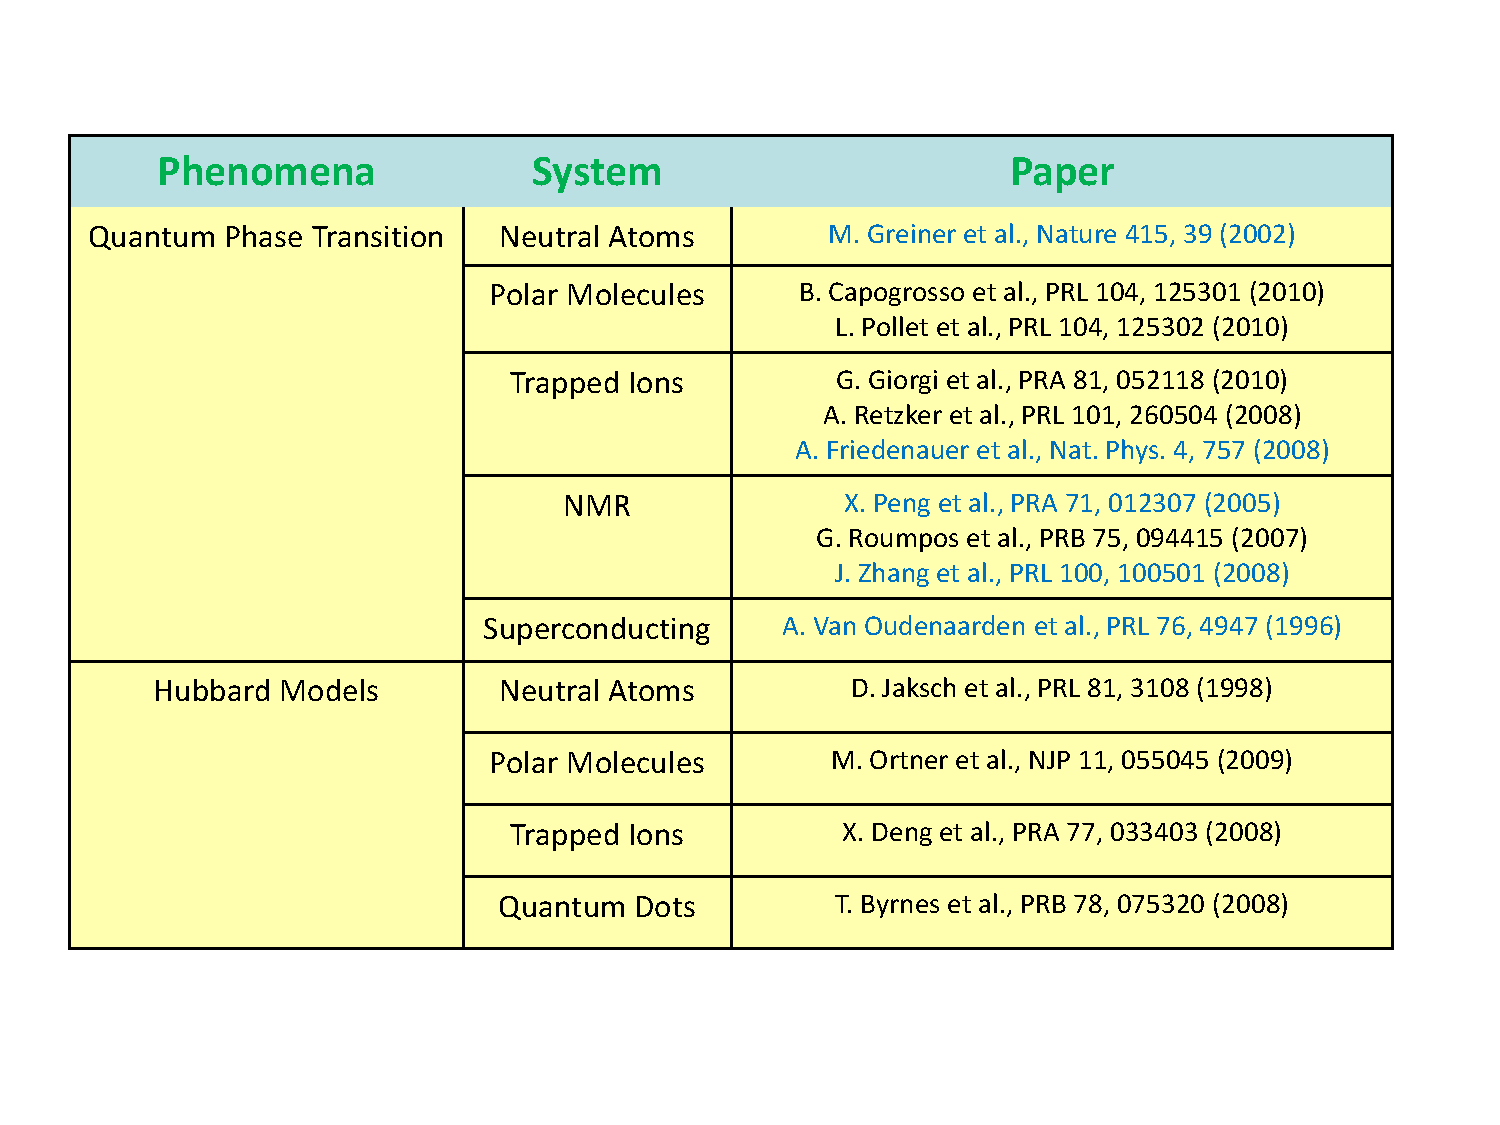
\includegraphics[width= 0.8\columnwidth]{figures/simcondense1.pdf}
              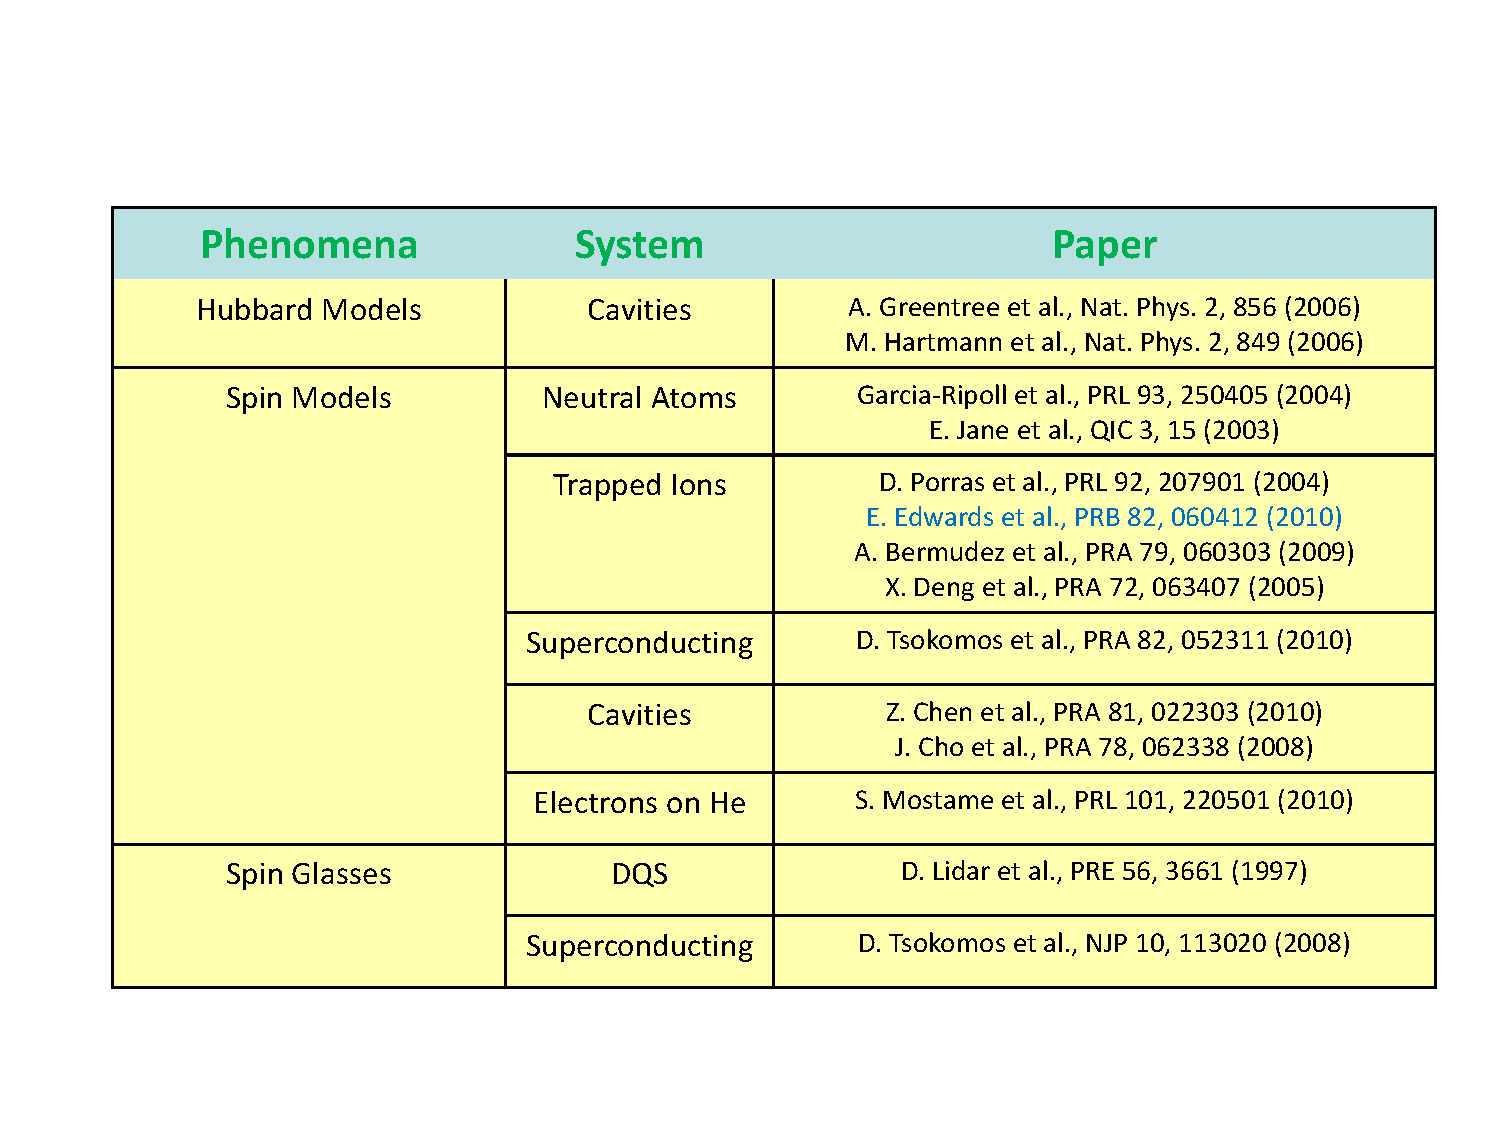
\includegraphics[width= 0.8\columnwidth]{figures/simcondense2.pdf}
              \caption{量子模拟在凝聚态物理中的应用(上)。蓝色字体为实验进展,黑色字体为理论进展。
              }
              \label{supersim}
            \end{center}
\end{figure}


\emph{4. 无序系统}

无序系统在凝聚态中的很多困难问题中出现,比如输运,传导,自旋玻璃,高温超导等等。而经典上关于无序系统的处理非常具有挑战性,因此有很多的量子模拟算法
被提出来。例如,Fano-Anderson模型的哈密顿量为
 \begin{equation}\label{supersim}
 H_{FA} = \sum_{l=1}^{n-1}\varepsilon_{k_l} c^{\dagger}_{k_l} c_{k_l}+\epsilon b^{\dagger}b+V(c^{\dagger}_{k_0}b+c_{k_0}b^{\dagger}),
\end{equation}
其中费米算符$c^{\dagger}_{k_l}(c_{k_l})$和$b^{\dagger}(b)$分别可以在导电模式和杂质中产生(湮灭)非自旋费米子。该模型已经在NMR上实验实现\cite{nmrsim4}。

而在AQS的方案中,光晶格可以实验实现无序系统且观测到Bose-glass相\cite{atomsim7};无序势阱中可以研究BEC的Anderson-like局域化\cite{atomsim6};
离子阱可以用来研究无序系统中的物理现象\cite{dis1};描述导电区的磁性杂质的哈密顿量则可以映射到超导线路\cite{supersim3}。

\emph{5. 高温超导}

包含氧化铜的复合物中的高温超导也是一个可以用量子模拟解决的难题。利用量子点我们可以用AQS的方式模拟高温超导体\cite{dotsim3},$t-J$模型也被证明可以被模拟\cite{high1}.
BCS对模型的哈密顿量则可以用DQS来模拟,其一般形式为
 \begin{equation}\label{supersim}
 H_{BCS} = \sum_{m=1}^{N} \frac{\epsilon}{2}(n_m^F+n_{-m}^N)+\sum_{m,l=1}^{N}V_{ml}^{+}c_m^{\dagger}c_{-m}^{\dagger}c_{-l}c_l,
\end{equation}
$c_m^{\dagger}(c_m)$和$b_m^{\dagger}(b_m)$分别为费米和玻色的产生(湮灭)算子,$|m|=1,2,\cdots,N$为量子数。实现该模型的量子模
拟算法\cite{high2}和NMR实验\cite{nmrsim6}目前也已完成。

\emph{6. 自旋玻璃}

如果自旋间的相互作用是铁磁或反铁磁的,即使在低温下空间内的自旋取向也不再是唯一的,而会呈现出一定的随机性,这种自旋玻璃的性质也可以用DQS模拟,
比如构造Ising模型中的Gibbs分布\cite{glass1}。该算法适用于任何维度的自旋玻璃Ising模型,或者含外磁场的模型。

用AQS的方法模拟Lipkin-Meshkov-Glick模型
 \begin{equation}\label{supersim}
 H_{LMG} = -\frac{\Delta}{2}\sum_{i=1}^{N} \sigma_i^z-\frac{J}{2}(\sum_{i=1}^{N}\sigma_i^x)^2+\frac{NJ}{2},
\end{equation}
以及复杂量子系统,比如Sherrington-Kirkpatrick自旋玻璃被Tsomokos等人给出\cite{glass2},而这个模型可以在超导线路中被自然模拟。

\emph{7. 超颖材料}

量子范畴的可控超颖材料的行为也可以被量子系统模拟\cite{meta1,supersim4}。量子超颖材料的一个例子是共振腔中全同qubit的无限链模型,这种系统中有可能实现
新的控制电磁场演化的方法,而这在经典材料里是完全做不到的。

\emph{8. 拓扑序}

任意子是量子统计性质既不满足玻色性也不满足费米性的二维粒子,可以用来描述石墨烯或量子霍尔效应等现象。而且,任意子可以被用作拓扑量子计算\cite{topo1}。
该模型既可以通过小尺度的DQS模拟\cite{topo2},也可以利用中性原子用AQS的方式模拟。前者在Lu等人的文章中已经用线性光学体系实验证实\cite{anyons1},其哈密顿量为
\begin{equation}\label{supersim}
 H_{K} = -\sum_vA_v-\sum_pB_p,
\end{equation}
其中$A_v=\prod_{i\in v}\sigma_i^x$和$B_p=\prod_{i\in p}\sigma_i^z$,$v$取遍所有顶点而$p$取遍所有平面。在光晶格中满足阿贝尔和非阿贝尔性质的任意子也可以通过
增加辅助粒子来实现,利用超导线路甚至可以构筑Kitaev蜂巢模型\cite{anyons2}。不仅对量子模拟,这些方案对拓扑量子计算的发展也有很大贡献。


\begin{figure}[htbp]
            \begin{center}
              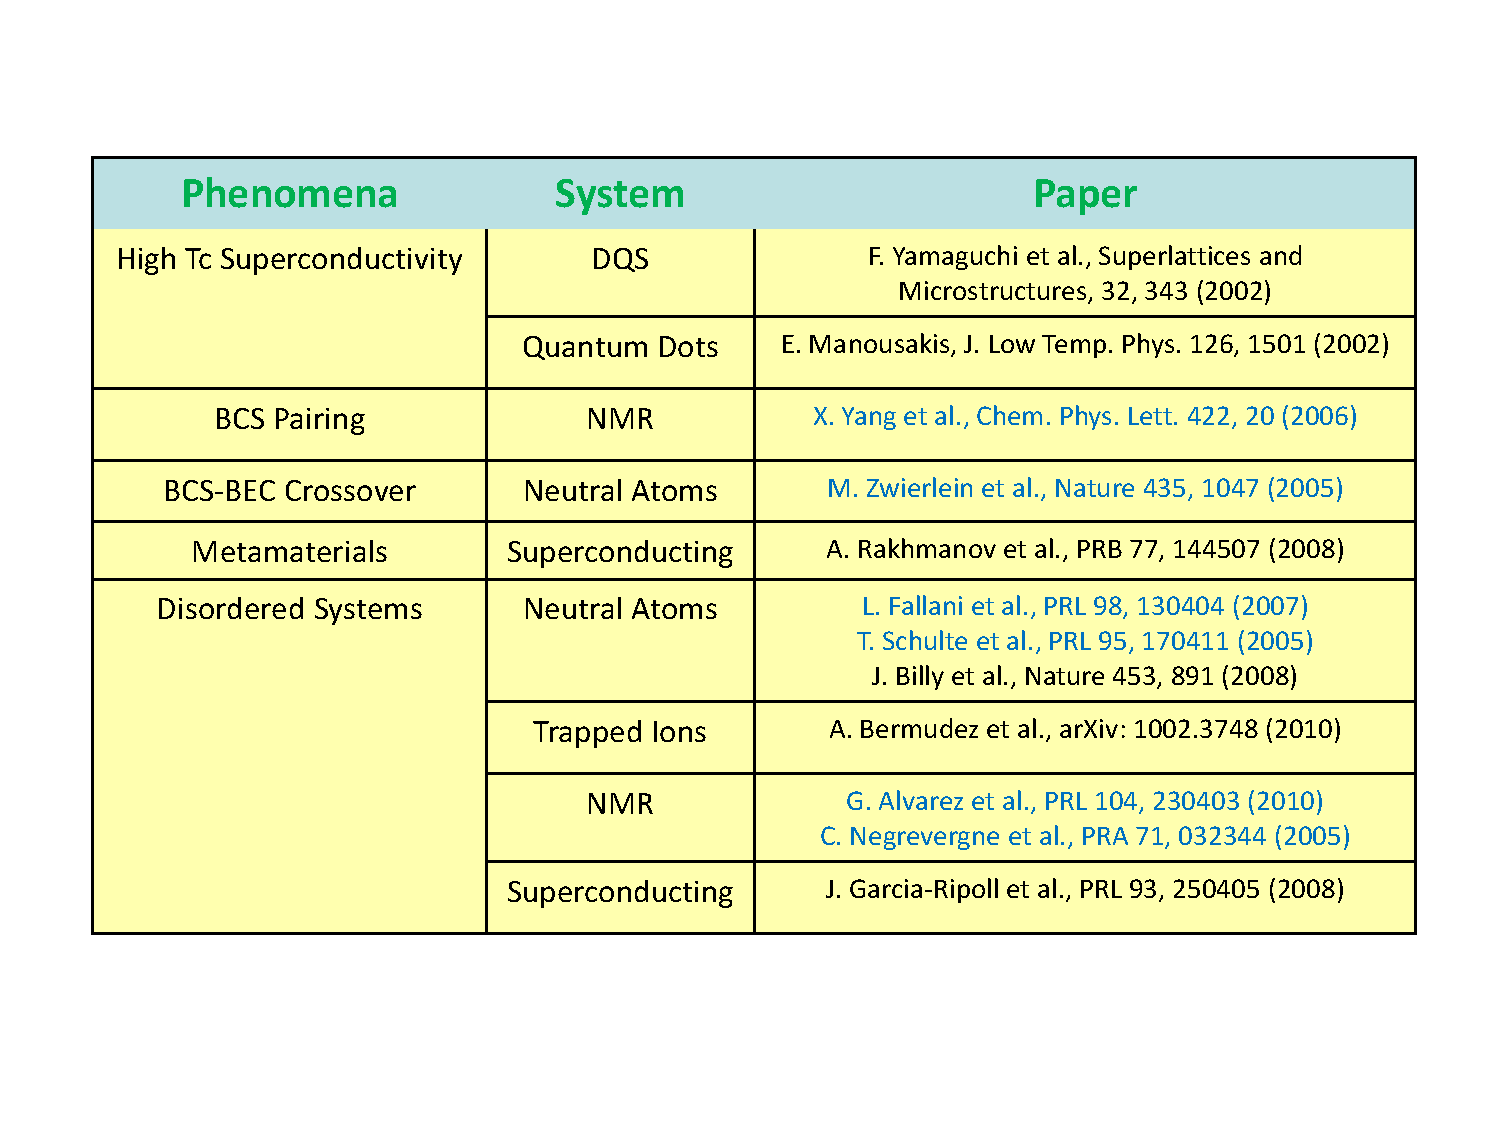
\includegraphics[width= 0.8\columnwidth]{figures/simcondense3.pdf}
              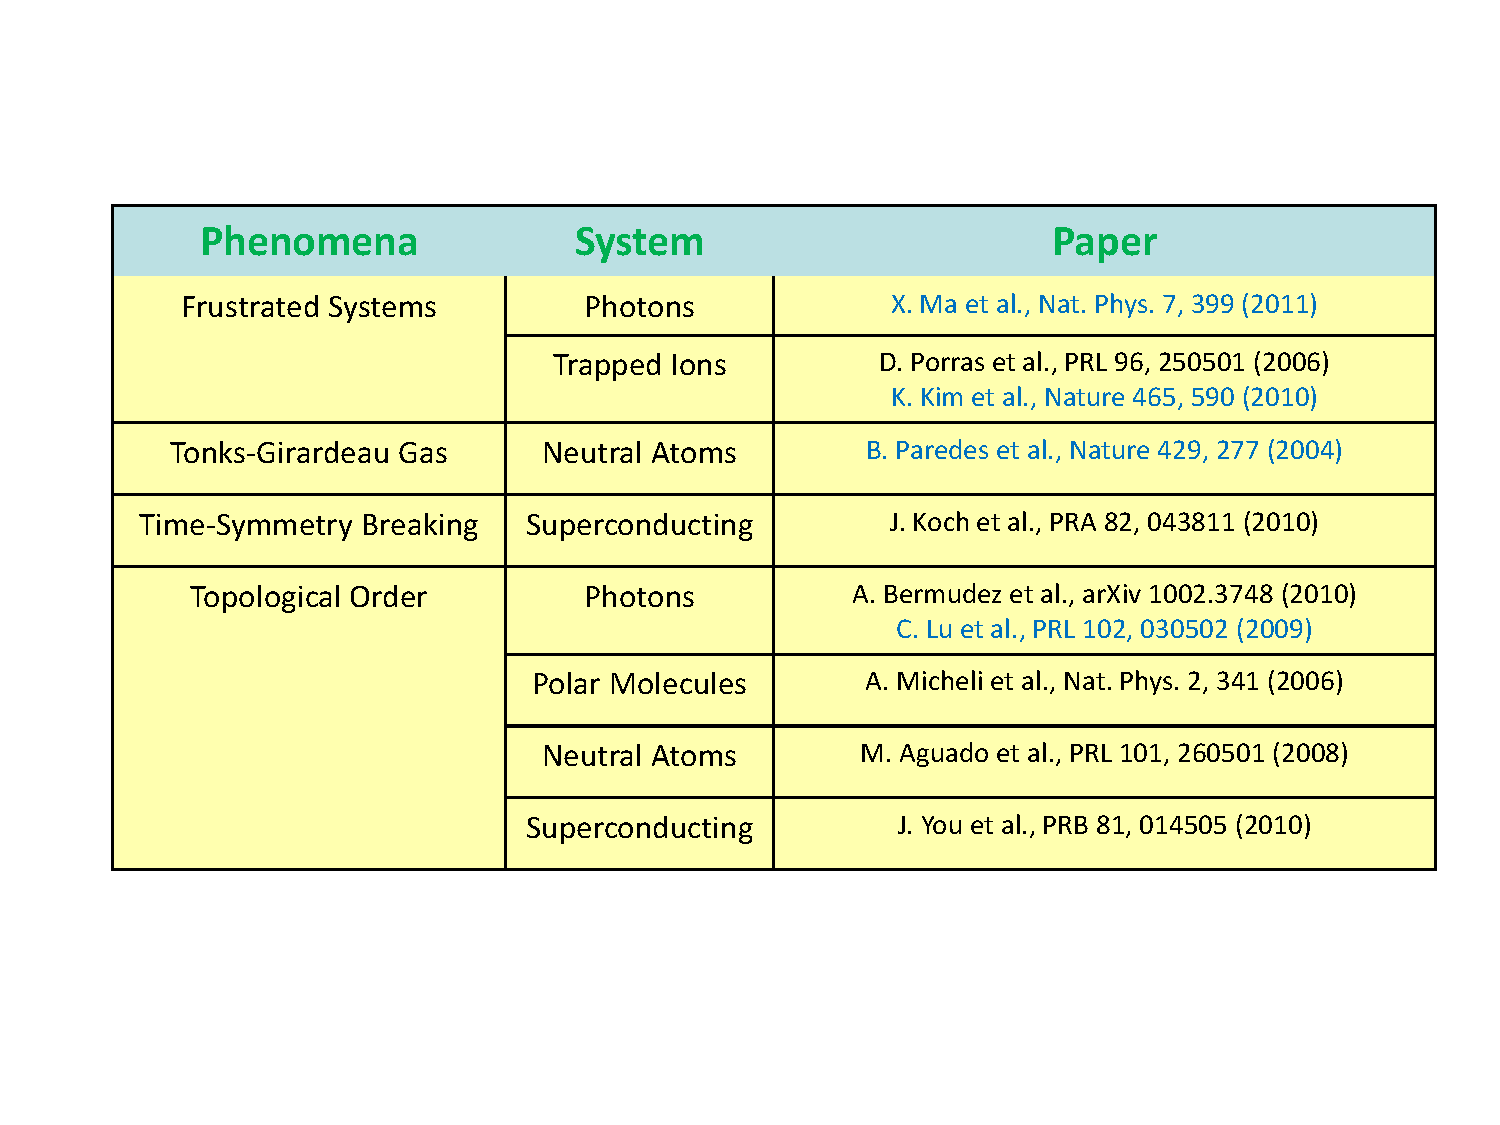
\includegraphics[width= 0.8\columnwidth]{figures/simcondense4.pdf}
              \caption{量子模拟在凝聚态物理中的应用(下)。蓝色字体为实验进展,黑色字体为理论进展。
              }
              \label{supersim}
            \end{center}
\end{figure}

  \subsection{高能物理}

量子模拟另外一个应用是在高能物理领域。第一次关于利用量子模拟研究相对论量子系统,例如规范场和Dirac费米子等的工作在1998年被提出\cite{energy1}
后来,陆续有其他一些模拟高能物理的理论和实验出现,比如如何建立2+1 Dirac振子和Jaynes-Cummings模型的映射\cite{dirac1},3+1维度模拟Dirac方程\cite{dirac2,dirac} ,最近扩展到了利用离子阱\cite{energy2}及光晶格\cite{energy3}研究外磁场中的Zitterbewegung。

模拟晶格规范理论也是量子多体中的困难问题之一。用DQS模拟晶格规范理论在Byrnes和Yamamoto的文章中已被详细讨论\cite{energy4},他们证明可以把$U(1), SU(2), SU(3)$中的晶格规范哈密顿量算符写成自旋算符的形式,因此就可以在DQS上模拟。该方案中需求的逻辑门数量和模拟晶格的总数呈一个线性到二次函数之间的某种函数关系,因此
是有效的。同时,初始化和测量和晶格尺度的关系也是类似的。

光晶格则可以用来作为AQS模拟ring-exchange模型\cite{energy5,energy6},其哈密顿量为
\begin{equation}\label{supersim}
 H_{RE} = K\sum_{plaquettes}(b_1^{\dagger}b_2b_3^{\dagger}b_4+b_4^{\dagger}b_3b_2^{\dagger}b_1-n_1n_2-n_3n_4)。
\end{equation}
这个哈密顿量可以用一个含两个态的原子实现:一个被囚禁在四角晶格内并用Bose-Hubbard模型实现,另一个被囚禁在平面晶格内。利用这个模型我们还可以模拟
一系列的强耦合哈密顿量,并且研究强关联系统的性质。
\begin{figure}[htbp]
            \begin{center}
              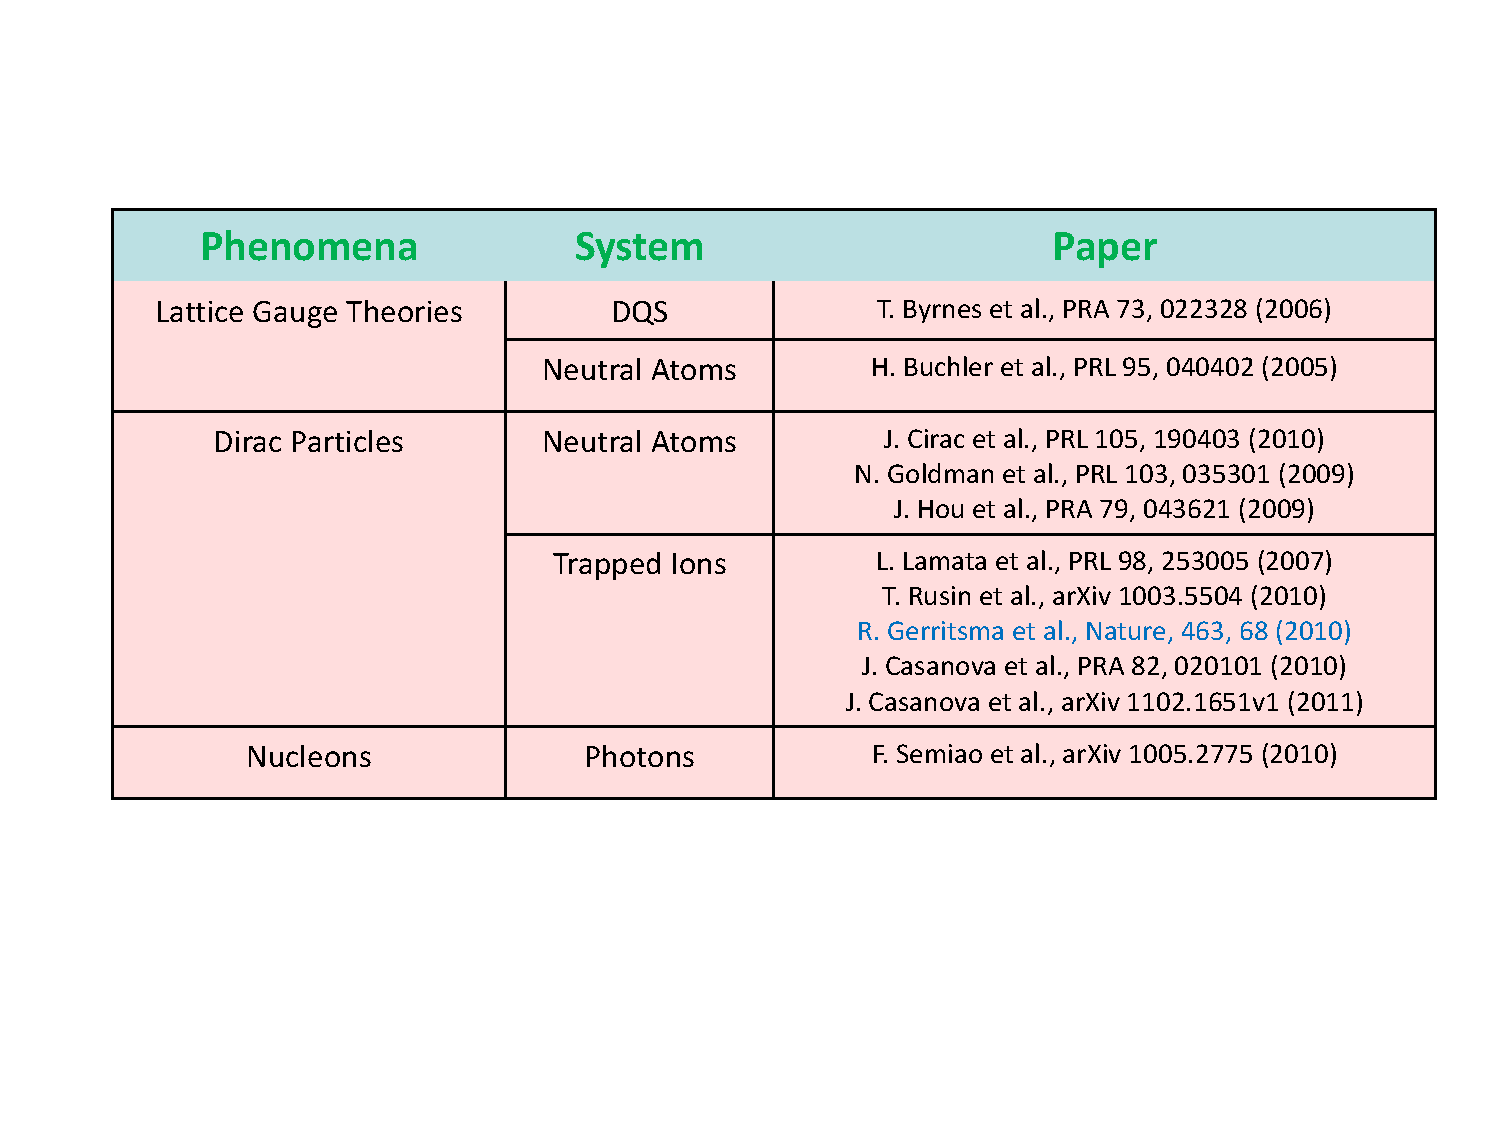
\includegraphics[width= 0.8\columnwidth]{figures/simhigh.pdf}
              \caption{量子模拟在高能物理中的应用。蓝色字体为实验进展,黑色字体为理论进展。
              }
              \label{simhigh}
            \end{center}
\end{figure}

此外,其他的方案还有利用光学体系模拟核子\cite{energy7}以及$O(3)$非线性介子模型\cite{energy8}等。

  \subsection{宇宙学}

量子模拟在万有引力理论以及宇宙学模型。例如利用BEC中的声波研究宇宙时空结构中的标量场\cite{cosmic},通过改变粒子内的耦合可以实现这个模拟过程。虽然
该方案在实验上很有挑战性,但它开辟了一条研究宇宙学的新道路。后来,利用AQS在离子阱中模拟宇宙粒子产生的方案\cite{cosmo1}及研究宇宙时空中的量子场效应的方案\cite{cosmo2}陆续出现。
利用AQS的方式,很有可能测试一些理论上有预言,但实验上尚未被观测到的现象,例如离子阱中的声子激发观测类Unruh效应\cite{unruh},或者光晶格中的中性原子
模拟Schwinger效应\cite{cosmo3},甚至Hawking辐射\cite{cosmo4,cosmo5}。

\begin{figure}[htbp]
            \begin{center}
              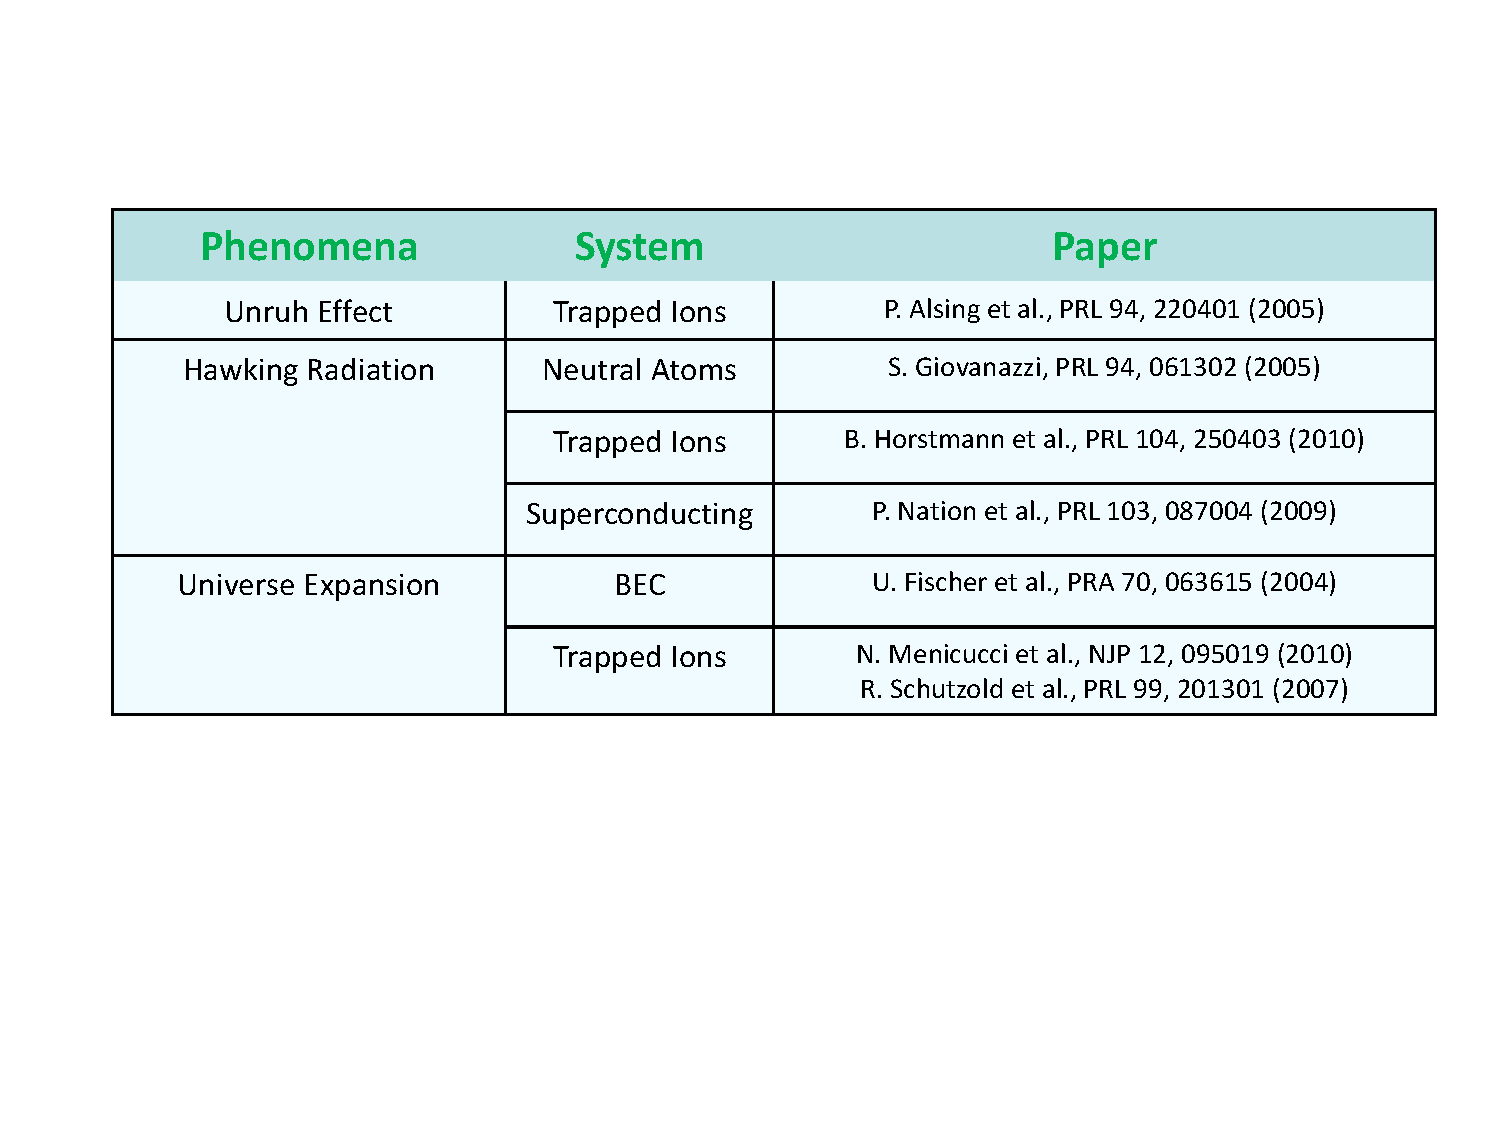
\includegraphics[width= 0.8\columnwidth]{figures/cosmic.pdf}
              \caption{量子模拟在宇宙学中的应用。蓝色字体为实验进展,黑色字体为理论进展。当然目前没有任何实验进展。
              }
              \label{cosmic}
            \end{center}
\end{figure}

 \subsection{原子物理}

原子物理及量子光学中最重要的模型之一是Jaynes-Cummings哈密顿量电磁场的单量子模式和两能级原子之间的相互作用,其形式为
\begin{equation}\label{supersim}
 H_{JC} = i\hbar g_0(a^{\dagger}\sigma_{-}-a\sigma_{+}),
\end{equation}
$g_0$是原子和场的耦合常数,$a^{\dagger}(a)$为玻色产生(湮灭)算符,而$\sigma_{+}(\sigma_{-})$为升(降)算子。

超导线路是非常适合实现Jaynes-Cummings哈密顿量模型的\cite{atomsim1}。超导线路非常适合模拟原子物理是因为
其行为非常类似于原子,或者叫“模拟原子”。和自然的原子相比,超导线路不需要采用可见光或微波
技术激发电子,而是通过电流、电压驱动这种激发过程。超导线路可以被特殊设计,比如极大的耦合项或者特定的跃迁频率,因此相对
真正的原子更有优势。在原子物理的现象中,除了模拟量子光学\cite{supersim5},超导线路还可以模拟边带冷却和科林斯王冷却(源于希腊神话的故事)\cite{atomsim2},
Landau-Zener-Stuckelberg干涉仪\cite{atomsim3}, Einstein-Podolsky-Rosen实验\cite{super2}等。

\begin{figure}[htbp]
            \begin{center}
              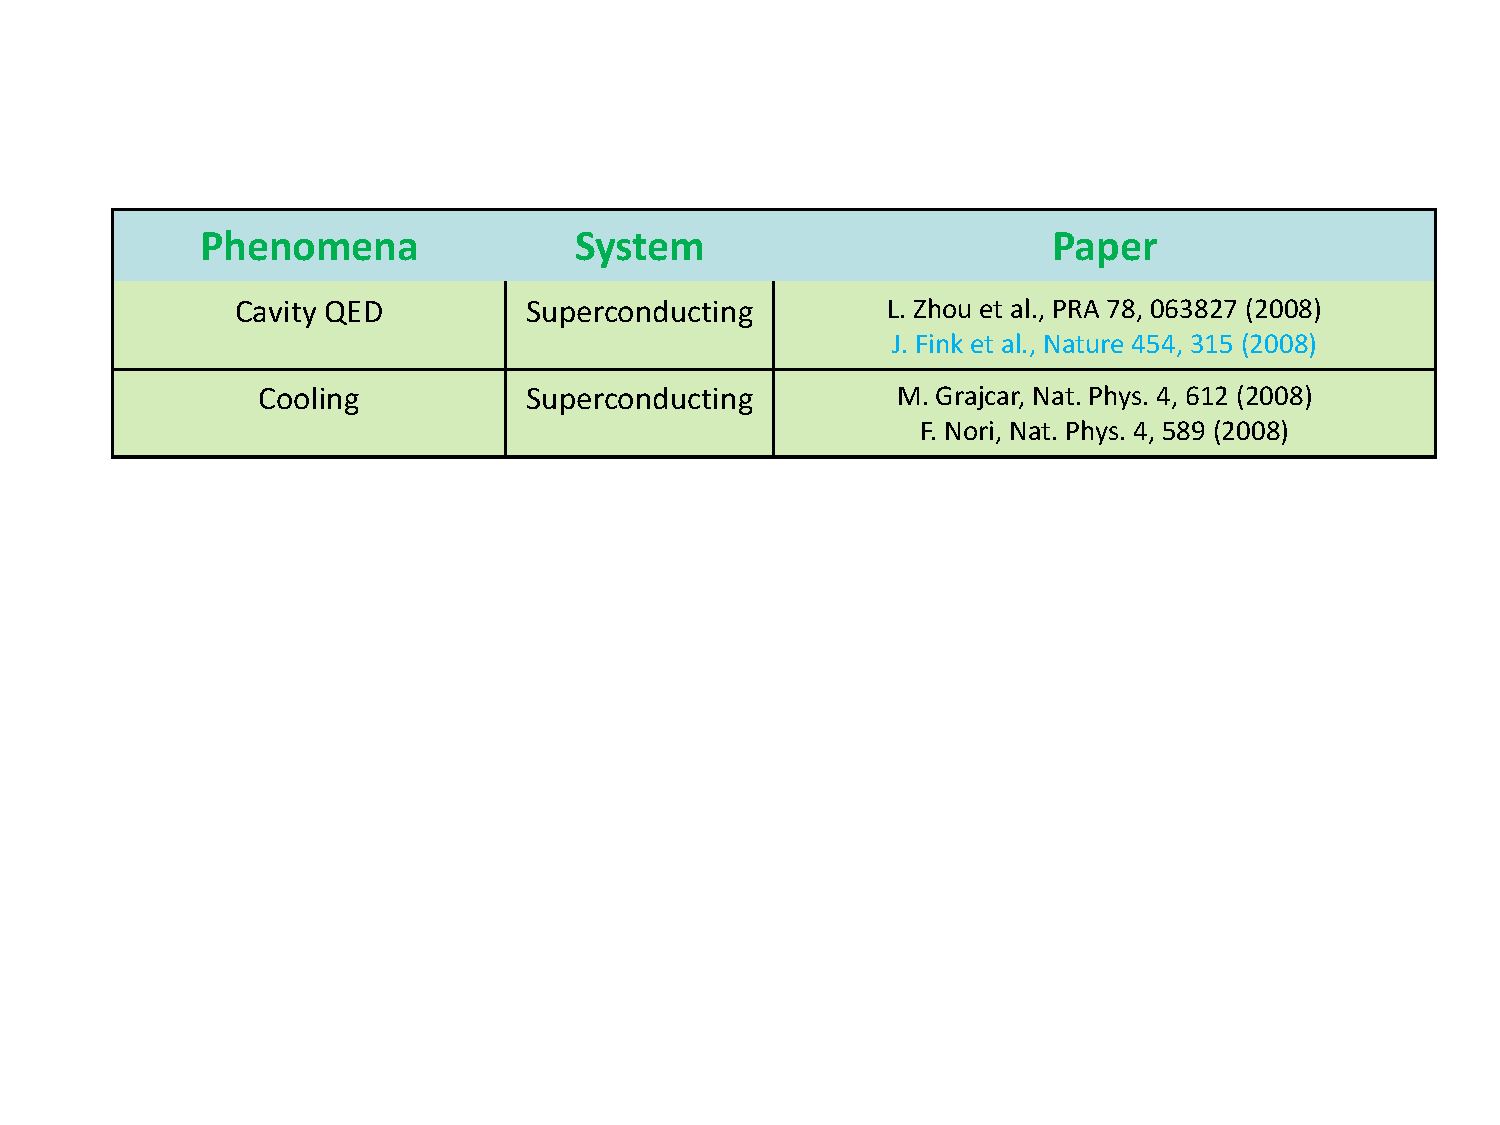
\includegraphics[width= 0.8\columnwidth]{figures/atomsim.pdf}
              \caption{量子模拟在原子物理中的应用。蓝色字体为实验进展,黑色字体为理论进展。
              }
              \label{atomsim}
            \end{center}
\end{figure}


 \subsection{量子化学}

量子模拟对量子化学也可以有很多贡献\cite{chem1}。在热反应速率常数的计算中\cite{chem2},首先把初态制备到所有位置本征态的等概率叠加态上,利用量子傅里叶变换
实现幺正演化,最后施加一系列测量并得到能量谱和幅度。该算法是多项式复杂度的,而在经典上要计算这个问题是指数复杂度的。

Aspuru-Guzik等人也提出可以利用DQS模拟分子的静态能级\cite{Alan_first}和动力学反应\cite{Polynomial_time_algorithm}。在模拟分子能级的过程中,qubit的数目是随着基矢数目的
增加呈线性增长的,而逻辑门的数目是多项式增长的,并证明利用几十个qubit我们就可以超越经典计算的结果。而在动力学模拟的过程中,该方案的复杂度也是多项式的。
这两个方案均已在实验上实现\cite{optics_static,static,dynamical}。这部分内容将在本论文的后面详细叙述,此处暂不作详细讨论。

用AQS也是可以模拟化学反应的。用可以视作“模拟原子”的量子点我们可以模拟多种化学反应\cite{reaction},最近还提出波导上的极冷原子也可以模拟化学反应过程\cite{chem3}。

\begin{figure}[htbp]
            \begin{center}
              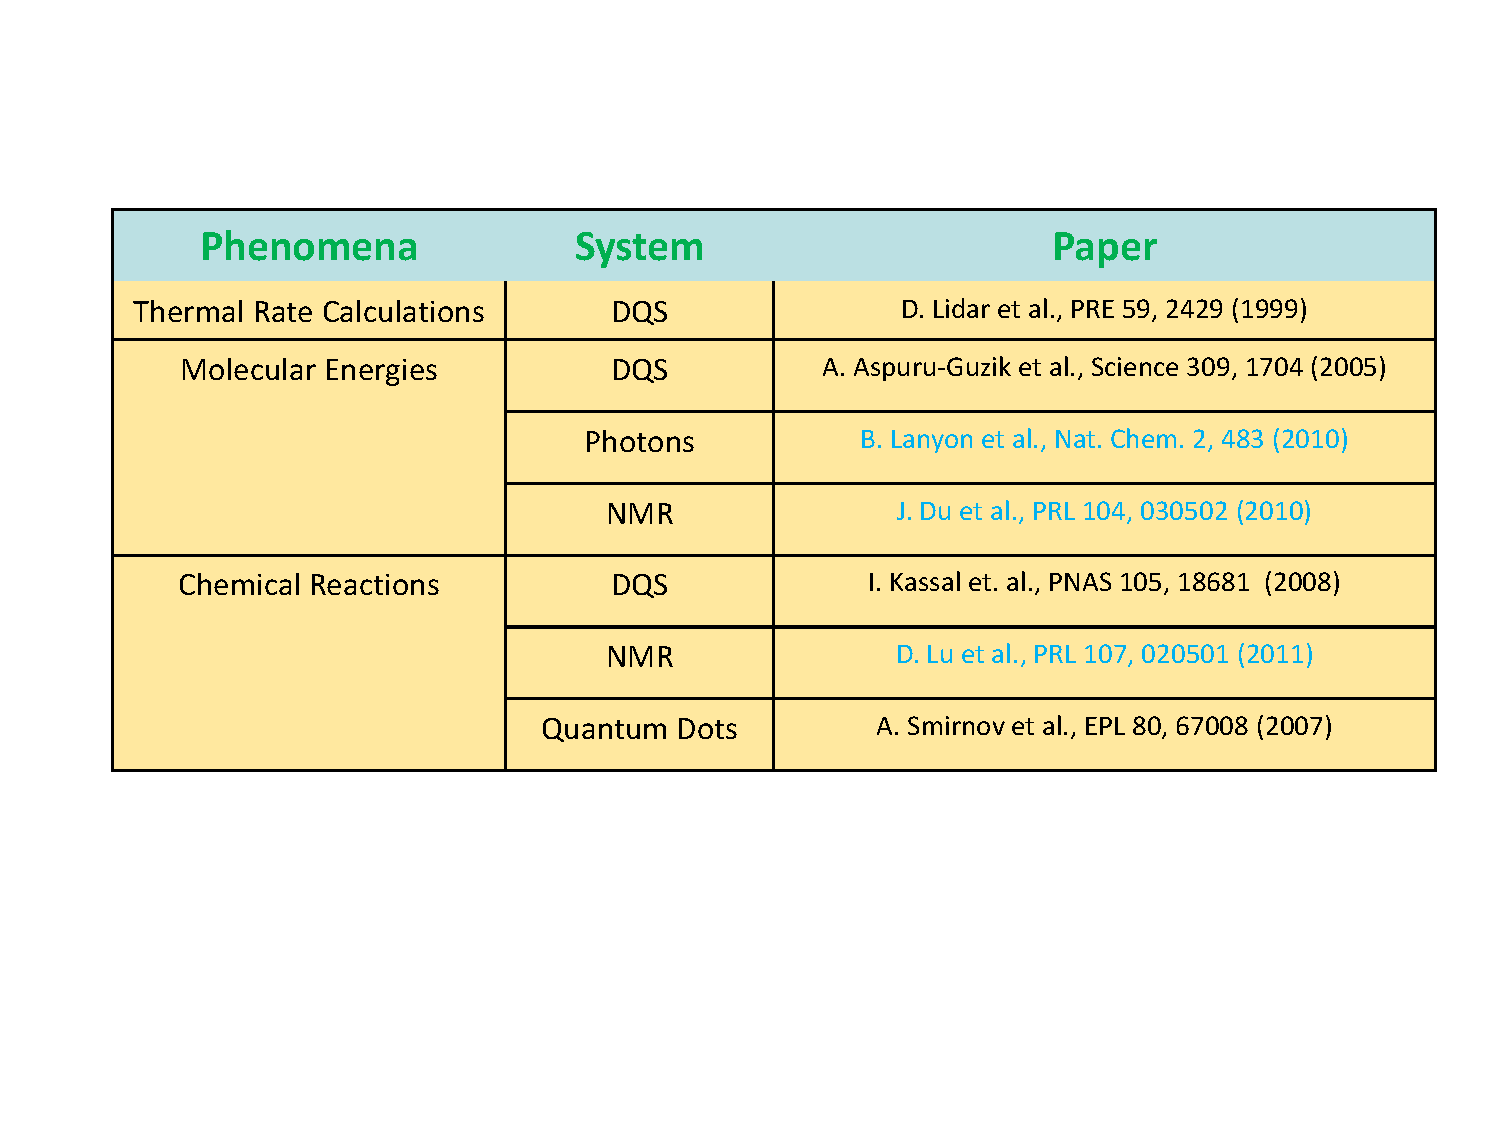
\includegraphics[width= 0.8\columnwidth]{figures/simchem.pdf}
              \caption{量子模拟在量子化学中的应用。蓝色字体为实验进展,黑色字体为理论进展。
              }
              \label{simchem}
            \end{center}
\end{figure}

 \subsection{开放系统}

模拟开放系统的动力学行为比封闭系统复杂很多,因为求解Lindblad方程需求的资源是求解薛定谔方程的二次方关系。模拟量子开放系统主要有两条路径:第一是通过利用实验
体系中天然的退相干机制\cite{Lloyd,deco}。第二条是利用封闭量子系统研究开放量子系统,例如利用驱动谐振子作为量子模拟器我们可以模拟非马尔科夫的阻尼谐振过程\cite{open1}。
模拟开放系统动力学机制的一般方法可以参见Bacon等的文章\cite{open2}。

\subsection{量子混沌}

DQS的一个应用就是用几个qubit研究简单量子映射的动力学过程,而量子面包师映射(quantum baker's map)是量子混沌中的典型问题。如果用量子模拟我们可以有效地解决这类问题,并在NMR\cite{chaos2}和线性光学\cite{chaos1}上已经被证实。
另外一个例子是kicked Harper模型\cite{chaos3}。在文章中的条件下,量子算法可以提供指数的加速,而且只用八个qubit就可以表现出非常有趣的性质。

\subsection{其它}

量子模拟的应用还有很多,比如利用DQS模拟薛定谔方程\cite{energy1,others1},量子热机\cite{others2,others3},量子热动力学\cite{others4}。现在量子模拟在物理和化学领域
都有非常多潜在的应用。利用量子模拟我们既可以解决一些经典上难以处理的问题(比如上面提到的凝聚态物理中的很多的问题),也可以实现一些实验非常困难甚至根本不能
做实验的难题(比如上面提到的高能物理和宇宙学中的一些问题)。随着技术的进步,肯定会有更多的学科希望加入到量子模拟的大军中来,也肯定会有更多新的应用将被展示。

\begin{figure}[htbp]
            \begin{center}
              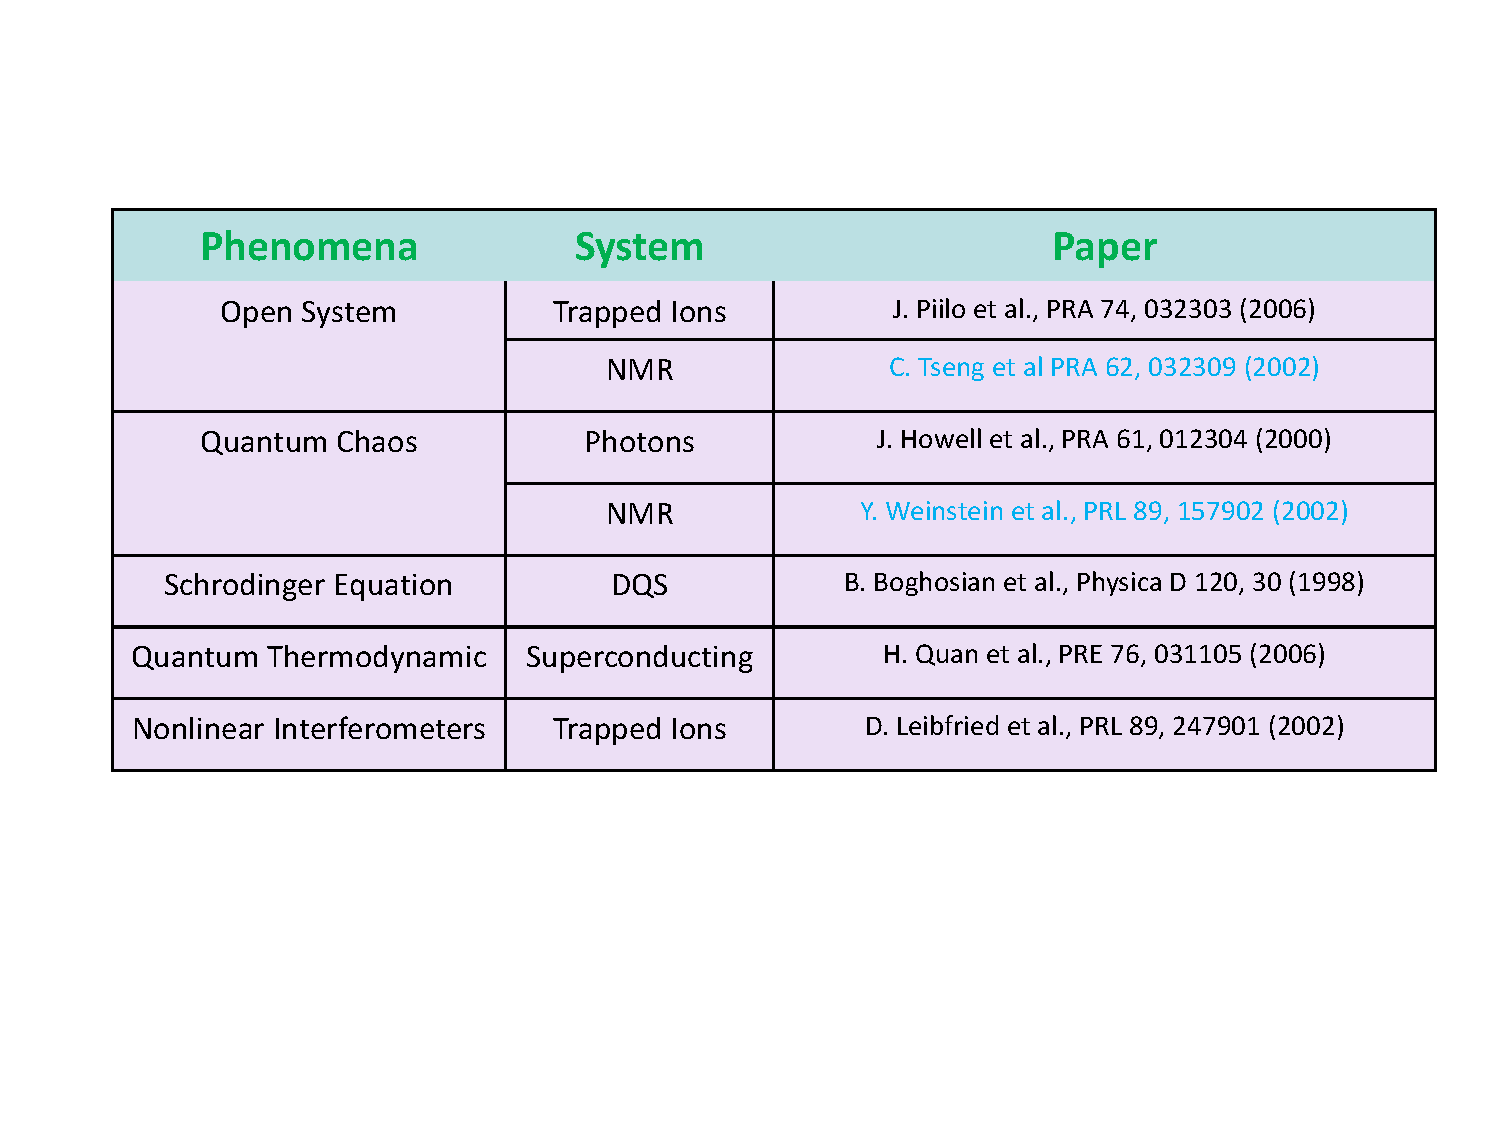
\includegraphics[width= 0.8\columnwidth]{figures/simother.pdf}
              \caption{量子模拟的一些相对“非主流”的应用。蓝色字体为实验进展,黑色字体为理论进展。
              }
              \label{simother}
            \end{center}
\end{figure}

\section{量子模拟的展望}

最近关于量子模拟的理论和实验进展让我们有理由期待在不远的未来一些特殊的量子模拟器能被建成。当然,理论和实验上还是有些问题要先克服的。

从理论的角度看,退相干和相干操控的研究依然是重点,同时对每个量子模拟器给出实验资源需求的估计也是必须的。量子模拟的新应用也是非常值得期待的,毕竟目前大多数的
方案和实验都在凝聚态物理上。

从实验的角度看,和量子计算机的要求类似,操控和可扩展性依然是两大难题。除了光晶格中的冷原子,其他的量子模拟目前还很难操控大的qubit阵列。尽管如此,光晶格中qubit
的单独控制和读出又是非常困难的,对其他体系这可能又不是一个很难的问题。目前还有绝热量子模拟的概念被提出\cite{adiaqs},这种新型的量子模拟器可能在实验上比基于逻辑门的DQS要简单。


\section{小结}

本章的主要内容是量子模拟。除了详细介绍量子模拟的概念及思想之外,本章也希望作为一个迄今为止比较完善的量子模拟资料库来使用,这对以后实验寻找新的、可行的量子模拟
方案有极大的便利之处。

\begin{figure}[htbp]
            \begin{center}
              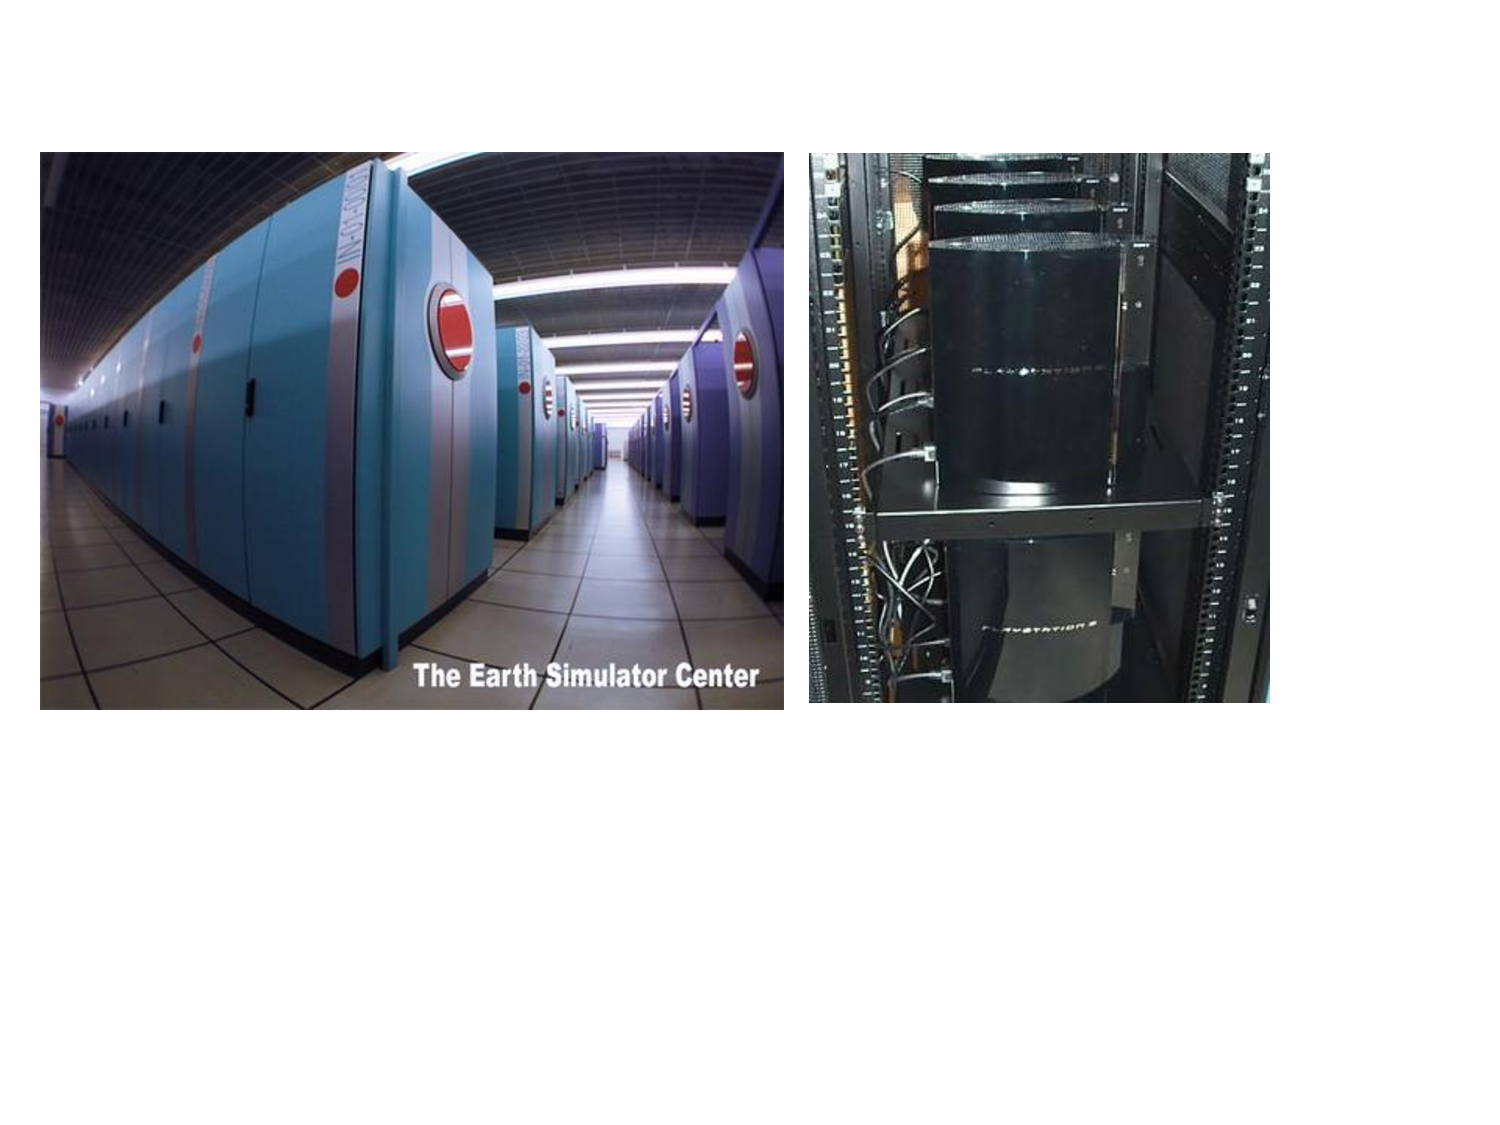
\includegraphics[width= 0.8\columnwidth]{figures/nec.pdf}
              \caption{(左) 日本电气公司(NEC)2002年开发的超级计算机“地球模拟器”。(右) PlayStation3被北卡罗来纳州立大学教授Frank Mueller做成阵列来跑计算,足见其计算能力之强,但离谣传的模拟地球依然差距不小。
              }
              \label{nec}
            \end{center}
\end{figure}

其实人类有一个很大的愿望就是成功模拟地球。早在2002年,日本电气公司(NEC)就为它研制的当时地球上最强大的超级电脑(比之前最快的IBM公司的ASCI White-Pacific快近五倍) 取了一个非常霸气的名字:地球模拟器(Earth Simulator)。当时这台电脑主要用于分析气候变化,当然不可能做到真正模拟地球上万物的演化。后来又有谣传说索尼(Sony)公司的新一代游戏主机PlayStation3可以强大到模拟地球,还一度愈演愈烈。
后来证实这只是一个半吊子的中日文翻译的问题。虽然目前看还不可能,但人类追逐梦想的脚步是从未停息的,而模拟地球应该是一个非常伟大的梦想。通过本章的介绍,我觉得我们可以怀有这种梦想:
量子模拟不仅只能用在凝聚态,高能物理,宇宙学,原子物理,量子化学上,它或者有着更加广阔的,更加不可思议的应用。当然目前我们最需要的依然是理论和实验上继续把这套思想完善下去,先开启“多个世界”的可能性。 